% !TEX program = pdflatex
% !TEX encoding = UTF-8 Unicode

% General TODO
% [ ] Remove `dedicatoria.tex`, we already have `agradecimientos.tex`
% [ ] Remove the use of apendixes, we are not using them yet
% [ ] In first two chapters, some vectors are not well typed, that's to say,
%     they're not in the form $\mathbf{v}$
% [ ] Use \observacion command when doing remarks
% TODO -- me quedo en la página 48 de mis notas
% TODO -- me quedo en la página 6 del paper

% Sergio Quijano Rey
% Doble Grado Ingenieria Informatica y Matematicas, UGR
% A partir de la plantilla dada en la página del grado de matemáticas de la UGR
% Dicha plantilla se puede descargar desde https://grados.ugr.es/informatica/pages/infoacademica/tfg/plantillas/plantilla_tfg_latex/!

% Usamos un documentclass propio del paquete KOMA-script
\documentclass{scrbook}

% Opciones del paquete KOMA-script
% Son las dadas por defecto en la plantilla, que sigue las directrices del TFG
\KOMAoptions{%
  fontsize=10pt,        % Tamaño de fuente
  paper=a4,             % Tamaño del papel
  headings=normal,      % Tamaño de letra para los títulos: small, normal, big
  parskip=half,         % Espacio entre párrafos: full (una línea) o half (media línea)
  headsepline=false,    % Una linea separa la cabecera del texto
  cleardoublepage=empty,% No imprime cabecera ni pie en páginas en blanco
  chapterprefix=false,  % No antepone el texto "capítulo" antes del número
  appendixprefix=false,	% No antepone el texto "Apéndice" antes de la letra
  listof=totoc,		    	% Añade a la tabla de contenidos la lista de tablas y figuras
  index=totoc,			    % Añade a la talba de contenidos una entrada para el índice
  bibliography=totoc,	  % Añade a la tabla de contenidos una entrada para bibliografía
  BCOR=5mm,           % Reserva margen interior para la encuadernación.
                        % El valor dependerá el tipo de encuadernado y del grosor del libro.
  DIV=10,             % Cálcula el diseño de página según ciertos
                        % parámetros. Al aumentar el número aumentamos el ancho de texto y disminuimos el ancho del margen. Una opción de 14 producirá márgenes estrechos y texto ancho.
}

% TODO -- mirar esto cuando vaya a imprimir el TFG
% INFORMACIÓN PARA LA VERSIÓN IMPRESA
% Si el documento ha de ser impreso en papel de tamaño a4 pero el tamaño del documento (elegido en \KOMAoptions con la ocpión paper) no es a4 descomentar la línea que carga el paquete `crop` más abajo. El paquete crop se encargará de centrar el documento en un a4 e imprimir unas guías de corte. El procedimiento completo para imprenta sería el siguiente:
% 0. Determinar, según el tipo de encuadernación del documento, el ancho reservado para el proceso de encuadernación (preguntar en la imprenta), es decir, la anchura del área del papel que se pierde durante el proceso de encuadernación. Fijar la varibale BCOR de \KOMAoptions a dicho valor.
% 1. Descomentar la siguiente línea e imprimir una única página con las guías de corte
% 2. Cambiar la opción `cross` por `cam` (o `off`) en el paquete crop y volver a compilar. Imprimir el documento (las guías de corte impresas no inferfieren con el texto).
% 3. Usar la página con las guías impresas en el punto 1 para cortar todas las páginas.

% \usepackage[a4, odd, center, pdflatex, cross]{crop} % Permite imprimir el documento en un a4 (si el tamaño es más pequeño) mostrando unas guías de corte. Útil para imprenta.

% ---------------------------------------------------------------------
%	PAQUETES
% ---------------------------------------------------------------------

% CODIFICACIÓN E IDIOMA
% ---------------------------------------------------------------------
\usepackage[utf8]{inputenc} 			    % Codificación de caracteres

% Selección del idioma: cargamos por defecto inglés y español (aunque este último es el idioma por defecto para el documento). Cuando queramos cambiar de idioma escribiremos:
% \selectlanguage{english} o \selectlanguage{spanish}

\usepackage[english, spanish, es-nodecimaldot, es-noindentfirst, es-tabla]{babel}

% Opciones cargadas para el paquete babel:
  % es-nodecimaldot: No cambia el punto decimal por una coma en modo matemático.
  % es-noindentfirst: No sangra los párrafos tras los títulos.
  % es-tabla: cambia el título del entorno `table` de "Cuadro" a "Tabla"

% Otras opciones del paquete spanish-babel:
  \unaccentedoperators % Desactiva los acentos en los operadores matemáticso (p.e. \lim, \max, ...). Eliminar esta opción si queremos que vayan acentuados

% MATEMÁTICAS
% ---------------------------------------------------------------------
\usepackage{amsmath, amsthm, amssymb} % Paquetes matemáticas
\usepackage{mathtools}                % Añade mejoras a amsmath
\mathtoolsset{showonlyrefs=true}      % sólo se numeran las ecuaciones que se usan
\usepackage[mathscr]{eucal} 					% Proporciona el comando \mathscr para
                                      % fuentes de tipo manuscrito en modo matemático sin sobreescribir el comando \mathcal

% TIPOGRAFÍA
% ---------------------------------------------------------------------
% El paquete microtype mejora la tipografía del documento.
\usepackage[activate={true,nocompatibility},final,tracking=true,kerning=true,spacing=true,factor=1100,stretch=10,shrink=10]{microtype}

% TODO -- para el codigo creo que es mejor fuente Cascadia Code (preferencia personal)
% Las tipografías elegidas para el documento, siguiendo la guía de estilo de la UGR,
% son las siguientes
% Normal font: 			URW Palladio typeface.
% Sans-serif font: 	Gill Sans
% Monospace font: 	Inconsolata
\usepackage[T1]{fontenc}
\usepackage[sc, osf]{mathpazo} \linespread{1.05}
\usepackage[scaled=.95,type1]{cabin} % sans serif in style of Gill Sans
% Si el paquete cabin da error usar el siguiente comando en su lugar
% \renewcommand{\sfdefault}{iwona}
\usepackage{inconsolata}


% Selecciona el tipo de fuente para los títulos (capítulo, sección, subsección) del documento.
\setkomafont{disposition}{\sffamily\bfseries}

% Cambia el ancho de la cita. Al inicio de un capítulo podemos usar el comando \dictum[autor]{cita} para añadir una cita famosa de un autor.
\renewcommand{\dictumwidth}{0.45\textwidth}

\recalctypearea % Necesario tras definir la tipografía a usar.

\usepackage{setspace}
% TABLAS, GRÁFICOS Y LISTADOS DE CÓDIGO
% ---------------------------------------------------------------------
\usepackage{booktabs}
% \renewcommand{\arraystretch}{1.5} % Aumenta el espacio vertical entre las filas de un entorno tabular

\usepackage{xcolor, graphicx}
% Carpeta donde buscar los archivos de imagen por defecto
\graphicspath{{img/}}

% IMAGEN DE LA PORTADA
% Existen varias opciones para la imagen de fondo de la portada del TFG. Todas ellas tienen en logotipo de la universidad de Granada en la cabecera. Las opciones son las siguientes:
% 1. portada-ugr y portada-ugr-color: diseño con marca de agua basada en el logo de la UGR (en escala de grises y color).
% 2. portada-ugr-sencilla y portada-ugr-sencilla-color: portada únicamente con el logotipo de la UGR en la cabecera.
\usepackage{eso-pic}
\newcommand\BackgroundPic{%
	\put(0,0){%
		\parbox[b][\paperheight]{\paperwidth}{%
			\vfill
			\centering
      % Indicar la imagen de fondo en el siguiente comando
			
\includegraphics[width=\paperwidth,height=\paperheight,%
			keepaspectratio]{portada-ugr-sencilla}%
			\vfill
}}}

% \usepackage{listings} % Para la inclusión de trozos de código

% CABECERAS
% ---------------------------------------------------------------------
% Si queremos modificar las cabeceras del documento podemos usar el paquete
% `scrlayer-scrpage` de KOMA-Script. Consultar la documentación al respecto.
% \usepackage[automark]{scrlayer-scrpage}

% VARIOS
% ---------------------------------------------------------------------

%\usepackage{showkeys}	% Muestra las etiquetas del documento. Útil para revisar las referencias cruzadas.

% ÍNDICE
% Para generar el índice hay que compilar el documento con MakeIndex. Generalmente los editores se encargan de ello automáticamente.
% ----------------------------------------------------------------------
% \index{} para añadir un elemento
% \index{main!sub} para añadir un elementos "sub" bajo la categoría "main".
% \index{termino|textbf} para dar formato al número de página (negrita).
% \index{termino|see{termino relacionado}} para crear una referencia cruzada

% Ejemplo: \index{espacio homogéneo}, \index{superficie!mínima}, \index{esfera|see{espacio homogéneo}}

% Activar los siguientes comandos para generar el índice terminológico. Ver también comandos al final de este documento para incluir dicho índice en el pdf final.
% \usepackage{makeidx}
% \makeindex

% Para revisar las entradas al índice conforme las incluimos en el documento es útil el siguiente paquete. Conviene observar que mientras esté cargado no se generará el índice.
%\usepackage{showidx} % Muestra en el margen del documento las entradas añadidas al índice. Útil para revisar el documento. Si está activo el índice no se genera

% == Mis librerias cargadas ==
%====================================================================================================

% Para poder escribir $\mathbb{}$
\usepackage{amssymb}
\usepackage{amsfonts}

% Para poder escribir matrices, vectores, ...
\usepackage{amsmath}

% Para poder cancelar terminos en las ecuaciones
\usepackage[makeroom]{cancel}

% Para poder usar \vv{x} para poner una flecha encima de x
\usepackage{esvect}

% Para hacer diagramas algebraicos
\usepackage{tikz}
\usepackage{tikz-cd}
\usetikzlibrary{tikzmark}
\usetikzlibrary{positioning}

% Para dejar notas en el documento
\usepackage{todonotes}

% Para poder poner varias imagenes en una unica figura
\usepackage{subcaption}

% Para fijar las figuras exactamente donde queramos
\usepackage{float}

% Porque voy a insertar fragmentos de codigo en el documento
\usepackage{listings}

% Para que los fragmentos de codigo acepte caracteres en utf8
\lstset{literate=
  {á}{{\'a}}1 {é}{{\'e}}1 {í}{{\'i}}1 {ó}{{\'o}}1 {ú}{{\'u}}1
  {Á}{{\'A}}1 {É}{{\'E}}1 {Í}{{\'I}}1 {Ó}{{\'O}}1 {Ú}{{\'U}}1
  {à}{{\`a}}1 {è}{{\`e}}1 {ì}{{\`i}}1 {ò}{{\`o}}1 {ù}{{\`u}}1
  {À}{{\`A}}1 {È}{{\'E}}1 {Ì}{{\`I}}1 {Ò}{{\`O}}1 {Ù}{{\`U}}1
  {ä}{{\"a}}1 {ë}{{\"e}}1 {ï}{{\"i}}1 {ö}{{\"o}}1 {ü}{{\"u}}1
  {Ä}{{\"A}}1 {Ë}{{\"E}}1 {Ï}{{\"I}}1 {Ö}{{\"O}}1 {Ü}{{\"U}}1
  {â}{{\^a}}1 {ê}{{\^e}}1 {î}{{\^i}}1 {ô}{{\^o}}1 {û}{{\^u}}1
  {Â}{{\^A}}1 {Ê}{{\^E}}1 {Î}{{\^I}}1 {Ô}{{\^O}}1 {Û}{{\^U}}1
  {ã}{{\~a}}1 {ẽ}{{\~e}}1 {ĩ}{{\~i}}1 {õ}{{\~o}}1 {ũ}{{\~u}}1
  {Ã}{{\~A}}1 {Ẽ}{{\~E}}1 {Ĩ}{{\~I}}1 {Õ}{{\~O}}1 {Ũ}{{\~U}}1
  {œ}{{\oe}}1 {Œ}{{\OE}}1 {æ}{{\ae}}1 {Æ}{{\AE}}1 {ß}{{\ss}}1
  {ű}{{\H{u}}}1 {Ű}{{\H{U}}}1 {ő}{{\H{o}}}1 {Ő}{{\H{O}}}1
  {ç}{{\c c}}1 {Ç}{{\c C}}1 {ø}{{\o}}1 {å}{{\r a}}1 {Å}{{\r A}}1
  {€}{{\euro}}1 {£}{{\pounds}}1 {«}{{\guillemotleft}}1
  {»}{{\guillemotright}}1 {ñ}{{\~n}}1 {Ñ}{{\~N}}1 {¿}{{?`}}1 {¡}{{!`}}1
}

% Para que los fragmentos de codigo no se salgan de los bordes y para fijar una fuente que resalte
\lstset{breaklines=true, basicstyle=\ttfamily}

% ---------------------------------------------------------------------
% COMANDOS Y ENTORNOS
% ---------------------------------------------------------------------
% Cargamos un archivo externo donde hemos incluido todos los comandos
% propios que vamos a usar en el documento.
% == Comandos de la plantilla ==
% ==============================================================================

\newcommand{\N}{\mathbb{N}}     % Naturales
\newcommand{\R}{\mathbb{R}}     % Reales
\newcommand{\Z}{\mathbb{Z}}     % Enteros
\newcommand{\Q}{\mathbb{Q}}     % Racionales
\newcommand{\C}{\mathbb{C}}     % Complejos

% TEOREMAS Y ENTORNOS ASOCIADOS

% \newtheorem{theorem}{Theorem}[chapter]:
\newtheorem*{teorema*}{Teorema}
\newtheorem{teorema}{Teorema}[chapter]
\newtheorem{proposicion}{Proposición}[chapter]
\newtheorem{lema}{Lema}[chapter]
\newtheorem{corolario}{Corolario}[chapter]

\theoremstyle{definition}
\newtheorem{definicion}{Definición}[chapter]
\newtheorem{ejemplo}{Ejemplo}[chapter]

\theoremstyle{remark}
\newtheorem{observacion}{Observación}[chapter]

% == Mis comandos propios ==
% ==============================================================================

% Comando que uso para expresar el conjunto {1, ..., param_1}
\newcommand{\deltaset}[1]{\Delta_{#1}}

% Comando que uso para expresar el conjunto {param_1, ..., param_2}
\newcommand{\doubledeltaset}[2]{\Delta_{#1}^{#2}}


% Espacio de matrices pxq
\newcommand{\espaciomatrices}[2]{\mathbb{M}_{#1 \times #2}}

% Espacio de tensores de orden N, #1 y de dimension M, #2 en cada modo
\newcommand{\espaciotensores}[2]{\mathcal{T}_{#1, #2}}

% Un mejor simbolo para QED
% Hago el renew para que \begin{proof} \end{proof} muestre este simbolo como a mi me gusta
\newcommand{\customqed}{\hfill\blacksquare}
\renewcommand{\qedsymbol}{$\customqed$}

% Elementos con explicaciones encima:

% Para poner cualquier cosa encima de otra dada
\newcommand{\encima}[2]{\ensuremath{\stackrel{#2}{#1}}}

% Igualdades
\newcommand{\eqtext}[1]{\ensuremath{\stackrel{\text{#1}}{=}}}
\newcommand{\eqmath}[1]{\ensuremath{\stackrel{#1}{=}}}

% Implicaciones
\newcommand{\impliestext}[1]{\ensuremath{\stackrel{\text{#1}}{\implies}}}

% Comando para indicar algun tipo de isomorfismo
\newcommand{\isomorfismo}[1]{\underset{#1}{\cong}}

% Expresiones logicas mas sencillas
\newcommand{\then}{\implies}
\newcommand{\iif}{\Longleftrightarrow}

% Algunos vectores que usamos bastante
\newcommand{\vectordd}[2]{\begin{pmatrix} #1 \\ #2 \end{pmatrix}}
\newcommand{\vectorn}[3]{\begin{pmatrix} #1 \\ #2 \\ \vdots \\ #3 \end{pmatrix}}

% Dos espacios
\newcommand{\dspace}{\ \ }

% Espacio de tensores de orden N (#1) y dimension M (#2) en cada modo
% TODO -- ahora estoy usando \espaciotensores que es mejor notacion
\DeclareMathOperator*{\MediumOtimes}{\text{\raisebox{0.25ex}{\scalebox{0.8}{$\bigotimes$}}}}
\newcommand{\esptensores}[2]{\overset{#1} \MediumOtimes \R^{#2}}

% (N)otacion para los (v)ectores => (nv)
% En el paper usan negrita, pero yo quiero usar una flechita encima
% Con este comand, si luego quiero cambiar la notación para los vectores (ie. volver
% a usar la notacion del paper) el cambio es sencillo
%
% NOTE: para poder usarse tiene que estar en un bloque de matematicas, por ejemplo:
% `$\nv{x}$`
\newcommand{\nv}[1]{\overrightarrow{#1}}

\newcommand{\entrecomillado}[1]{\textit{``#1''}}

% Forma mas comoda para escribir el producto escalar
\newcommand{\innerproduct}[2]{\langle #1 \; | \; #2 \rangle}

% Para añadir comentarios debajo o encima de elementos de una formula
\newcommand{\comentardebajo}[2]{\underbrace{#1}_\textrm{#2}}
\newcommand{\comentarencima}[2]{\overbrace{#1}^\textrm{#2}}

% Comando para evitar que las captions de las subfiguras colisionen entre si
\newcommand{\ajustarsubcaptions}{\captionsetup[subfigure]{width=0.9\textwidth,position=b}}

% Comando para escribir conjuntos matematicos
\newcommand{\conjunto}[1]{\{ #1 \}}

% Para escribir union e interesccion
\newcommand{\interseccion}{\bigcap}
\newcommand{\union}{\bigcup}

% Para hacer `\to` pero de forma larga, como con \longmapsto
\newcommand{\longto}{\longrightarrow}

% Para hacer el conjunto de combinaciones lineales `span`
% Cuidado porque hay un comando de latex que ya se llama span
\newcommand{\spansetlong}[2]{\text{span}_{#1} \conjunto{#2}}
\newcommand{\spanset}[1]{\spansetlong{\mathbb{R}}{#1}}

% El paquete `cleveref` usa los nombres de secciones en ingles, los necesito
% en español
\Crefname{section}{Sección}{Sección}
\crefname{section}{Sección}{Sección}
\Crefname{chapter}{Capítulo}{Sección}
\crefname{chapter}{Capítulo}{Capítulo}

% Comandos para referenciar
\newcommand{\imgref}[1]{\Cref{#1}}
\newcommand{\sectionref}[1]{\Cref{#1}}
\newcommand{\coderef}[1]{\Cref{#1}}
\newcommand{\tableref}[1]{\Cref{#1}}
\newcommand{\propref}[1]{\Cref{#1}}

% Deberiamos evitar el uso de este comando generico
\newcommand{\customref}[1]{\Cref{#1}}


% --------------------------------------------------------------------
% INFORMACIÓN DEL TFG Y EL AUTOR
% --------------------------------------------------------------------
\usepackage{xspace} % Para problemas de espaciado al definir comandos

% TODO -- hay que poner un titulo al trabajo
% TODO -- hay que poner informacion de los tutores
\newcommand{\miTitulo}{Título del trabajo\xspace}
\newcommand{\miNombre}{Sergio Quijano Rey\xspace}
\newcommand{\miGrado}{Doble Grado en Ingeniería Informática y Matemáticas}
\newcommand{\miFacultad}{Facultad de Ciencias, Escuela Superior Ingeniería Informática y Telecomunicaciones}
\newcommand{\miUniversidad}{Universidad de Granada}

% Añadir tantos tutores como sea necesario separando cada uno de ellos
% mediante el comando `\medskip` y una línea en blanco
\newcommand{\miTutor}{
    Javier Merí de la Maza \\ \emph{Departamento de Análisis Matemático}

    \medskip
    Pablo Mesejo Santiago \\ \emph{Departamento de Ciencias de la Computación e Inteligencia Artificial}

    \medskip
    Guillermo Gómez Trenado \\ \emph{Departamento de Ciencias de la Computación e Inteligencia Artificial}
}
\newcommand{\miCurso}{2022-2023\xspace}

% HYPERREFERENCES
% --------------------------------------------------------------------
\usepackage{xurl}
\usepackage{hyperref}
% Opciones para el paquete hyperref
%----------------------------------

\hypersetup{%
  % hidelinks,            % Enlaces sin color ni borde. El borde no se imprime
  linkbordercolor=0.8 0 0,
  citebordercolor=0 0.8 0,
  citebordercolor=0 0.8 0,
  colorlinks = true,            % Color en texto de los enlaces. Comentar esta línea o cambiar `true` por `false` para imprimir el documento.
  linkcolor = [rgb]{0.5, 0, 0}, % Color de los enlaces internos
  urlcolor = [rgb]{0, 0, 0.5},  % Color de los hipervínculos
  citecolor = [rgb]{0, 0.5, 0}, % Color de las referencias bibliográficas
	pdftitle={\miTitulo},%
	pdfauthor={\textcopyright\ \miNombre, \miFacultad, \miUniversidad},%
  pdfsubject={Trabajo de fin de Grado},%
	pdfkeywords={},%
	pdfcreator={pdfLaTeX},%
}

% Redefinición del estilo para mostrar las referencias cruzadas en la bibliografía.
% \renewcommand*{\backref}[1]{}
% \renewcommand{\backrefsep}{, }
% \renewcommand{\backreftwosep}{ y }
% \renewcommand{\backreflastsep}{ y }
% \renewcommand*{\backrefalt}[4]{{\footnotesize [%
%     \ifcase #1 No citado%
%     \or Citado en pág.~#2%
%     \else Citado en págs. #2%
%     \fi%
% ]}}

% Etiquetas en español para el comando \autoref
\def\chapterautorefname{Capítulo}
\def\appendixautorefname{Apéndice}
\def\sectionautorefname{Sección}
\def\subsectionautorefname{Subsección}
\def\figureautorefname{Fig.}
\def\tableautorefname{Tabla}

\def\teoremaautorefname{Teorema}
\def\proposicionautorefname{Proposición}
\def\lemaautorefname{Lema}
\def\corolarioautorefname{Corolario}
\def\definicionautorefname{Def.}
\def\observacionautorefname{Observación}
\def\ejemploautorefname{E.j.}

% Pone automáticamente un parántesis para las ecuaciones
\def\equationautorefname~#1\null{(#1)\null}


\begin{document}

% --------------------------------------------------------------------
% FRONTMATTER
% -------------------------------------------------------------------
\frontmatter % Desactiva la numeración de capítulos y usa numeración romana para las páginas

% \pagestyle{plain} % No imprime cabeceras

% !TeX root = ../libro.tex
% !TeX encoding = utf8

%*******************************************************
% Titlepage
%*******************************************************
\begin{titlepage}
  \AddToShipoutPicture*{\BackgroundPic}
  \phantomsection
  \pdfbookmark[1]{Título}{title}

  % Para que el título esté centrado en la página.
  % Los valores numéricos deberán elegirse de acuerdo con el diseño de
  % página (sobre todo si se cambia la opción BCOR o DIV).
  \begin{addmargin}[2.575cm]{0cm}
  \begin{flushleft}
    \Large
    \hfill\vfil

    \large{\textsf{\miFacultad}}
    \vfill

    {\large\textsc\miGrado} \vfill


    {\large\textsc{trabajo de fin de grado}}

    \begin{flushleft}
      \Huge
      \setstretch{0.8}
      \miTitulo
    \end{flushleft}

    \vfill\vfill\vfill\vfill

    \textsf{\normalsize{Presentado por:}}\\
    {\normalsize\textrm{\miNombre}}
    \bigskip

    \textsf{\normalsize{Tutores:}}\\
    {\normalsize\rmfamily\miTutor}

    \bigskip
    \textsf{\normalsize{Curso académico \miCurso}}
  \end{flushleft}
  \end{addmargin}

\end{titlepage}
\cleardoublepage
\endinput

% !TeX root = ../libro.tex
% !TeX encoding = utf8

%*******************************************************
% Little Dirty Titlepage
%*******************************************************

\thispagestyle{empty}

\begin{center}
  \large  

  \vspace*{\stretch{1}}

  \begingroup
  \huge{\miTitulo} \\ \bigskip
  \endgroup

  \textrm{\miNombre}

  \vspace{\stretch{5}}

\end{center}  

\newpage
\thispagestyle{empty}

\hfill

\vfill

\miNombre \textit{\miTitulo}.

Trabajo de fin de Grado. Curso académico \miCurso.
\bigskip

\begin{minipage}[t]{0.25\textwidth}
  \flushleft
  \textbf{Responsable de tutorización}
\end{minipage}
\begin{minipage}[t]{0.45\textwidth}
  \flushleft
  \miTutor
\end{minipage}
\begin{minipage}[t]{0.30\textwidth}
  \flushright
  \miGrado
  \medskip

  \miFacultad
  \medskip

  \miUniversidad
\end{minipage}

\newpage
\endinput

% !TeX root = ../libro.tex
% !TeX encoding = utf8
%
%*******************************************************
% Declaración de originalidad
%*******************************************************

\thispagestyle{empty}

\hfill\vfill

\textsc{Declaración de originalidad}\\\bigskip

D./Dña. \miNombre \\\medskip

Declaro explícitamente que el trabajo presentado como Trabajo de Fin de Grado (TFG), correspondiente al curso académico \miCurso, es original, entendida esta, en el sentido de que no ha utilizado para la elaboración del trabajo fuentes sin citarlas debidamente.
\medskip

En Granada a \today 
\begin{flushleft} 
Fdo: \miNombre 

\end{flushleft}

\vfill

\cleardoublepage
\endinput

% !TeX root = ../libro.tex
% !TeX encoding = utf8

%*******************************************************
% Dedication
%*******************************************************
\thispagestyle{empty}
\phantomsection 
\pdfbookmark[1]{Dedicatoria}{Dedicatoria}

\hfill
\vfill

\begin{flushright}
\itshape
Dedicatoria (opcional) \\
Ver archivo \texttt{preliminares/dedicatoria.tex}
\end{flushright}

\vfill

\cleardoublepage
\endinput
                % Opcional
% !TeX root = ../libro.tex
% !TeX encoding = utf8

%*******************************************************
% Table of Contents
%*******************************************************
\phantomsection
\pdfbookmark[0]{\contentsname}{toc}

\setcounter{tocdepth}{2} % <-- 2 includes up to subsections in the ToC
\setcounter{secnumdepth}{3} % <-- 3 numbers up to subsubsections

% \manualmark
% \markboth{\textsc{\contentsname}}{\textsc{\contentsname}}
\tableofcontents

% Sergio: modifico este archivo para que se incluyan en el indice las figuras, tablas y codigos


%*******************************************************
% List of Figures and of the Tables
%*******************************************************

    % *******************************************************
    %  List of Figures
    % *******************************************************
    % \phantomsection
    \listoffigures

    %*******************************************************
    % List of Tables
    %*******************************************************
    % \phantomsection
    \listoftables

    %*******************************************************
    % List of Listings
    % The package \usepackage{listings} is needed
    %*******************************************************
      % \phantomsection
    \renewcommand{\lstlistlistingname}{Listados de código}
    \lstlistoflistings

\cleardoublepage

% !TeX root = ../libro.tex
% !TeX encoding = utf8

%*******************************************************
% Agradecimientos
%*******************************************************

\chapter{Agradecimientos}

Agradecimientos del libro (opcional, ver archivo \texttt{preliminares/agradecimiento.tex}).

\cleardoublepage
\endinput
            % Opcional

% \pagestyle{scrheadings} % A partir de ahora sí imprime cabeceras

% !TeX root = ../libro.tex
% !TeX encoding = utf8
%
%*******************************************************
% Summary
%*******************************************************

% TODO -- lo tengo que escribir, porque es una parte obligatoria

\selectlanguage{english}
\chapter{Summary}

\todo{Escribirlo cuando la parte de informática se estabilice algo}

An english summary of the project (around 800 and 1500 words are recommended).

File: \texttt{preliminares/summary.tex}


% Al finalizar el resumen en inglés, volvemos a seleccionar el idioma español para el documento
\selectlanguage{spanish}
\endinput

% !TeX root = ../libro.tex
% !TeX encoding = utf8
%
%*******************************************************
% Introducción
%*******************************************************

% \manualmark

% \markboth{\textsc{Introducción}}{\textsc{Introducción}}

\chapter{Resumen}

% 1. Objetivos
% 1. Papers principales con los que trabajamos
% 1. Objetivos alcanzados y objetivos no alcanzados
% 1. Estado del arte

\textbf{Palabras clave}: Análisis Tensorial, Descomposición Tensorial \textit{CP}, Descomposición Tensorial \textit{HT}, Aprendizaje Automático, Aprendizaje Profundo, Visión por Computador, Redes Convolucionales, Reconocimiento Facial Invariante a la Edad, \textit{Triplet Loss}

El presente Trabajo de Fin de Grado tiene dos \textbf{objetivos principales}. El primero de ellos consiste en realizar una modelización de las redes neuronales convolucionales, profundas y no profundas, y estudiar la propiedad conocida comúnmente como \textit{depth efficiency}. El segundo objetivo consiste en resolver una tarea de reconocimiento facial invariante a cambios en la edad. Además, estudiaremos ciertas variantes sobre la función de pérdida \textit{Triplet Loss}, buscando resolver algunos problemas asociados al uso de esta técnica. Dichas variantes suponen un gran esfuerzo de implementación, por lo tanto, buscamos aplicar patrones de diseño para que la arquitectura resultante sea fácil de modificar y extender.

El uso de técnicas de aprendizaje automático basado en redes neuronales profundas ha crecido enormemente en los últimos años. Su buen rendimiento en ciertas tareas específicas ha sido demostrado de forma contundente. Sin embargo, este buen rendimiento \textbf{se justifica únicamente sobre la evidencia experimental}. No se realizado un estudio profundo y fructífero sobre los motivos teóricos que respaldan los resultados experimentales. Los trabajos que realizan un estudio para respaldar la línea experimental suelen trabajar con modelizaciones matemáticas alejadas de los modelos comunes del \textit{deep learning}, y los resultados suelen tratar sobre casos concretos en los que las redes profundas son claramente superiores a las redes no profundas o \textit{shallow}. La publicación con la que trabajamos principalmente es \cite{matematicas:principal}.

Nuestro trabajo en esta línea es novedoso por dos motivos principales: la \textbf{modelización matemáticas de las redes neuronales es muy cercana a la realidad}, y el resultado sobre \textbf{\textit{depth efficiency} da información concreta sobre la cantidad de escenarios} en los que ocurre esta \textit{depth efficiency}.

Expresaremos las funciones de puntuación que la red busca aprender en base a un tensor de coeficientes sobre una base de funciones linealmente independientes y totales. A partir de aquí, la modelización se basa en dos conocidas descomposiciones tensoriales, la descomposición \textit{CANDECOMP/PARAFAC} o \textit{CP} y la descomposición jerárquica \textit{Tucker} o \textit{HT}. Estas \textbf{modelizaciones tienen en cuenta las propiedades fundamentales de las redes convolucionales}: localidad de la convolución, compartición de coeficientes y operadores de \textit{pooling}.

Demostraremos \textbf{dos resultados centrales}. El primero nos muestra que, en el sentido de la medida de Lebesgue, casi todos los modelos no profundos necesitan un número exponencial de parámetros para implementar un modelo profundo. El segundo resultado añade que, de hecho, casi todos los modelos profundos no pueden ni siquiera ser aproximados por un modelo no profundo con menos de un número exponencial de parámetros.

En esta línea, \textbf{los objetivos de este estudio han sido alcanzados}. Hemos presentado una modelización matemática muy cercana a la realidad, y hemos demostrado dos resultados que nos dan información exacta sobre en qué escenarios son superiores las redes profundas frente a las redes no profundas, y cómo de frecuente sucede esto.

Por otro lado, hemos \textbf{intentado resolver una tarea de reconocimiento facial invariante a la edad, o \textit{AIFR}}. Esta tarea resulta muy interesante en el ambiente de la \textbf{informática forense}, por todas las aplicaciones prácticas que tiene obtener un modelo capaz de identificar a un individuo en distintas imágenes independientemente de la edad con la que aparezca en dichas imágenes. Buscamos aplicar las técnicas introducidas en la publicación \cite{informatica:principal} en la tarea de \textit{AIFR}, enfoque que según nuestro conocimiento nunca se había aplicado a esta tarea.

Dicha tarea presenta una complejidad elevada. Además de los retos que supone una tarea de visión por computador usual, debemos añadir todos los \textbf{retos asociados a cómo el envejecimiento afecta las características faciales} con las que trabajamos.

Para resolver el problema planteado, realizamos un estudio del estado del arte, que nos indica las principales líneas de trabajo que más éxito han tenido. Estos trabajos utilizan principalmente redes generativas adversarias para descomponer los datos de entrada en dos características incorreladas: edad e identidad. Algunos trabajos utilizando modelos basados en atención para aprender a resolver esta tarea. Este enfoque usa técnicas y modelos avanzados, que quedan fuera del alcance del presente trabajo.

Realizamos un estudio de los conjuntos de datos disponibles. Estos son escasos y en ocasiones de una calidad pobre. Estudiamos el tamaño de los conjuntos de datos, las distribuciones del número de imágenes por individuo (fundamental para aplicar nuestras técnicas), la distribución de edad de los individuos y la distribución del rango de edad de los individuos. En base a este estudio tomamos una decisión informada de qué conjuntos usar y qué protocolo experimental aplicar. Siguiendo la línea más común en el estado del arte, entrenamos sobre un conjunto de datos grande, \textit{CACD}, y validamos sobre el conjunto \textit{FG-Net}, que presenta un gran reto por su gran variedad en edades y rangos.

Desarrollamos una amplia base de código para poder aplicar las técnicas estudiadas. Realizamos una optimización de la base de código guíada por los datos tomados durante varios \textit{profiles}, debido a necesidades de rendimiento. Por los malos resultados obtenidos, aplicamos una amplia \textit{suite} de \textit{tests} para validar que los malos resultados no estén provocados por fallos en la implementación.

Realizamos una \textbf{experimentación y estudio de los resultados}. Eston son pésimos, muy lejos de ser competitivos con el estado del arte y, todavía peor, muy lejanos de ser aplicables en un escenario práctico. El estado del arte obtiene valores para \textit{Rank@1 Accuracy} superiores al 90\%. Nuestro modelo no llega al 0.1\%. Además, al no existir literatura concreta sobre el uso de estas técnicas sobre un problema de \textit{AIFR}, debemos justificar los pésimos resultados en base al presente trabajo.

Por lo tanto, \textbf{se ha cumplido el objetivo de desarrollar una base de código bien diseñada}, con la que sea cómodo trabajar y experimentar. Sin embargo, los \textbf{resultados experimentales son muy malos y quedan muy lejos de los objetivos propuestos} inicialmente.

\endinput


% --------------------------------------------------------------------
% MAINMATTER
% --------------------------------------------------------------------
\mainmatter % activa la numeración de capítulos, resetea la numeración de las páginas y usa números arábigos

\setpartpreamble[c][0.75\linewidth]{
    % Deja un espacio vertical en la parte superior
	\bigskip

    En esta primera parte del trabajo, introduciremos dos modelizaciones matemáticas muy cercanas a los modelos reales que se usan en la práctica del aprendizaje automático. Un modelo será no profundo (\entrecomillado{shallow})  y otro será profundo. Demostraremos que los modelos profundos son más eficientes que los modelos no profundos.
}
\part{Primera parte}

\chapter{Introducción}\label{ch:introduccion}

El objetivo de este trabajo, desde la perspectiva de las matemáticas, es \textbf{analizar las redes neuronales profundas basadas en convoluciones y explicar por qué en ciertos escenarios éstas funcionan mejor que las redes neuronales no profundas}, a las que llamaremos redes someras. En este escenario ocurre que para replicar redes profundas con un número polinomial de coeficientes, necesitamos que las redes someras tengan un número de coeficientes superior al polinomial, concretamente, exponencial. En este caso hablamos de \textbf{eficiencia en profundidad} o \textbf{\entrecomillado{depth efficiency}}.
\todo{Poner aquí una referencia a otra parte del paper sobre esto de tamaño exponencial}

La eficiencia en profundidad es muy conocida en la práctica, pero pocos son los trabajos que han tratado de justificar matemáticamente por qué ocurre este fenómeno. Además, como se comenta en \cite{matematicas:principal}, \textbf{en la mayoría de trabajos de este tipo, no se han tenido en cuenta propiedades fundamentales de las redes profundas ni de las redes convolucionales} \cite{matematicas:paper_depth_malo_01} \cite{matematicas:paper_depth_malo_02} \cite{matematicas:paper_depth_malo_03}. Por otro lado, suelen ser trabajos en los que \textbf{se muestran ejemplos concretos} de funciones implementables (de forma eficiente) con redes profundas pero no con redes someras, sin dar \textbf{ningún tipo de información sobre con qué frecuencia ocurre esto}. En base a esto, las \textbf{principales fortalezas de este trabajo respecto a otros} es que consideramos:
\todo{Comentarios de JMeri: este tipo de afirmaciones pueden llevar a preguntas del tribunal. Preparar bien las posibles respuestas}
\todo{Quizás yo añadir comentarios sobre esta afirmación para que se responda automáticamente al leer esto}

\begin{itemize}
	\item La diferencia jerárquica entre ambos tipos de redes.
	\item Propiedades fundamentales de las redes convolucionales: compartición de los coeficientes en las convoluciones, localidad de la operación de convolución y uso de la operación de \textit{pooling}.
	\item Un estudio de lo frecuente que es tener funciones que sean implementables (de forma eficiente) por redes profundas pero no por redes someras.
\end{itemize}
\todo{Desarrollar más qué significan estas propiedades. En la introducción del paper se explica esto más o menos}

\section{Objetivos}

Los principales \textbf{objetivos} del presente trabajo son los siguientes. Como punto de partida, modelar matemáticamente la tarea de aprendizaje representando los datos de entrada, la tarea a resolver y el espacio de hipótesis en el que buscaremos la mejor solución. Posteriormente, modelar los dos tipos de redes neuronales (profundas y someras) a través de dos tipos de descomposiciones tensoriales. La descomposición \textit{CP}, que equivale al uso de redes someras y que desarrollamos en la \sectionref{subs:descomposcion_cp}. Y la descomposición \textit{HT}, que equivale al uso de redes profundas y que introducimos en la \sectionref{subs:descomposicion_ht}. Finalmente, demostrar dos resultados centrales que pondrán de manifiesto la superioridad de las redes profundas, en lo que se conoce como eficiencia en profundidad, a través de las ya mencionadas descomposiciones tensoriales.

El primer resultado central, el \propref{teorema:teorema_principal_especificacion}, dice que si tenemos un modelo profundo con un número polinomial de coeficientes, el modelo somero necesitará al menos un número exponencial de coeficientes para poder implementar el mismo modelo. Esto ocurre casi por doquier respecto al espacio de los coeficientes que determinan el modelo profundo. El segundo resultado central, el \propref{corolario:corolario_principal_concreto}, indica que no es que un modelo somero no pueda realizar el modelo profundo con menos de un número exponencial de parámetros, sino que no es capaz ni de aproximar al modelo profundo con menos de un número exponencial de parámetros. De nuevo, esto ocurre casi por doquier respecto al espacio de los coeficientes que determinan el modelo profundo.

Nos basaremos principalmente en el trabajo \cite{matematicas:principal}. Algunas de las herramientas que usaremos serán la teoría básica sobre tensores, las descomposiciones tensoriales \textit{CP} y \textit{HT}, la matrización de tensores, algunos resultados conocidos sobre la medida de Lebesgue y finalmente el álgebra de matrices básica.

\section{Estructura del trabajo}

La estructura del trabajo será la siguiente. En primer lugar, en el \sectionref{ch:matematicas_fundamentales} introduciremos las herramientas básicas sobre las que fundamentaremos nuestro trabajo. En concreto, introduciremos el concepto de producto tensorial. En segundo lugar, en el \sectionref{ch:tarea_aprendizaje} indicaremos cómo representamos matemáticamente la tarea de aprendizaje. Para ello, modelizaremos un espacio de hipótesis general, para lo cual justificaremos la elección de ciertas funciones de puntuación, que serán clave en el desarrollo del trabajo, y la elección de determinadas funciones de representación. En la \sectionref{subs:capa_de_representacion} daremos un primer paso común en la modelización de ambas arquitecturas de aprendizaje automático, presentando la primera capa de ambos modelos. En tercer lugar, en el \sectionref{ch:modelizacion} desarrollaremos las dos modelizaciones (somera y profunda) a partir de dos descomposiciones tensoriales (\textit{CP} y \textit{HT}, respectivamente). Veremos en ambos casos cómo las modelizaciones realizadas se corresponden con arquitecturas usadas en la práctica del aprendizaje automático. Compararemos el número de parámetros que definen cada modelo, pues será fundamental en nuestros resultados teóricos. En cuarto lugar, en el \sectionref{chapter:teoremas_y_demostraciones} introduciremos los dos resultados principales, veremos y demostraremos algunos resultados previos necesarios para las demostraciones y probaremos el teorema y corolario principal. En quinto y último lugar, en el \sectionref{chapter:conclusiones_trabajo_futuro} comentaremos los resultados obtenidos a partir del presente trabajo e introduciremos posibles líneas de estudio en base a nuestros resultados.

\chapter{Fundamentos teóricos} \label{ich:fundamentos_teoricos}

En esta sección introduciremos algunos \textbf{conceptos teóricos} sobre los que se basará nuestro trabajo, y por tanto, conviene conocer para entender este trabajo.

\section{\textit{Embeddings}} \label{isec:embeddings}

Nuestro trabajo busca desarrollar un modelo de aprendizaje automático que aprenda un \textit{embedding}. Un \textit{embedding} no es más que un mapeo desde un cierto espacio $X$ de datos de entrada (en nuestro caso, podemos considerar $X$ como el espacio de imágenes en las que aparecen caras) a un espacio vectorial $\R^N$. En la mayoría de casos, la dimensión del espacio de llegada $N$ es menor que la dimensión del espacio $X$.

Más formalmente, buscamos aprender una función

\begin{equation}
\begin{split}
    f_{\theta}: X & \to \R^N \\
    x & \mapsto f_{\theta}(x)
\end{split}
\end{equation}

que tomamos de una familia paramétrica de funciones $\{f_{\theta}: \theta \in \Theta \}$. En el caso de nuestro problema, podemos pensar en la familia de los modelos profundos de redes convolucionales ($\theta$ estaría por tanto compuesto por todos los coeficientes que determinan dicho modelo convolucional, luego podríamos pensar en $\Theta \subseteq \R^M$ donde $M$ es el número de coeficientes del modelo).

El criterio para escoger una función u otra de mapeo es que este deberá ser \textbf{semántico}. En el espacio de llegada $\R^N$ tenemos una métrica:

\begin{equation}
\begin{split}
    D: X \times X & \to [0, \infty) \\
    x, y & \mapsto D(x, y)
\end{split}
\end{equation}

Por ejemplo, la métrica euclídea. Queremos que \textbf{datos semánticamente relacionados en $X$ sean mapeados a vectores en $\R^N$ cercanos} por la métrica que fijemos. Del mismo modo, datos semánticamente distintos deberán ser mapeados a vectores distantes.

Además, será deseable que $f_{\theta}$ sea una función continua (en casi cualquier ámbito podemos considerar $X = \R^M$ para algún valor de $M$). Por ejemplo, en el caso de las imágenes, un ligero cambio en un \textit{píxel} de la imagen no debería producir un vector muy distanciado del original. En muchas ocasiones, al estar buscando que el \textit{embedding} sea semántico, esta restricción inducirá en menor o mayor medida dicha continuidad.

\begin{ejemplo}
    Consideremos que queremos computar un \textit{embedding} para representar palabras.

    Este problema es \textbf{especialmente relevante} en el ámbito del lenguaje natural. Esto es así porque, si queremos trabajar con texto usando modelos de aprendizaje automático, deberemos primero convertir dicho texto a una representación numérica. Usar, por ejemplo, el código binario que codifica dicho texto no parece muy buena idea, porque este mapeo no es semántico ni continuo.

    En este caso, queremos que palabras con una semántica parecida se transformen a vectores cercanos. Por ejemplo, la distancia entre los \textit{embeddings} de las palabras \entrecomillado{ciudad}, \entrecomillado{pueblo} debería ser mucho menor que la distancia entre los \textit{embeddings} de las palabras \entrecomillado{papel}, \entrecomillado{odio}. Esta idea se puede visualizar en la siguiente representación:

    \begin{figure}[H]
        \centering
        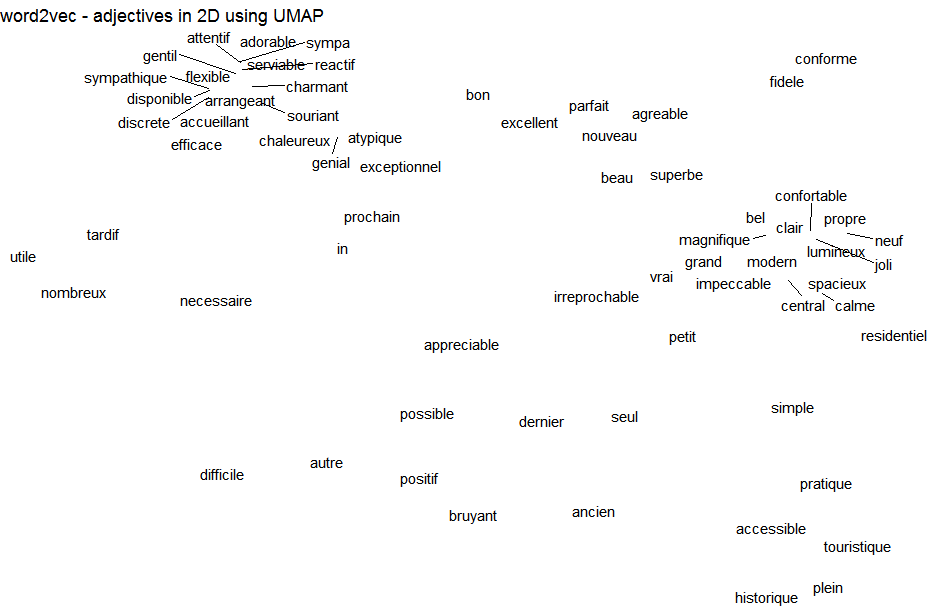
\includegraphics[width=0.6\textwidth]{informatica/word2vec_example}
        \caption{Ejemplo de un \textit{embedding} semántico, computado por el modelo \textit{word2vec} \cite{informatica:word2vec}, de palabras en francés. Imagen extraída de \url{https://cran.r-project.org/web/packages/word2vec/readme/README.html}}
    \end{figure}

    En el caso concreto de \cite{informatica:word2vec}, que propone el conocido modelo \textit{word2vec}, se consigue que el \textit{embedding} tenga cierta \entrecomillado{estructura algebraica}, pudiendo computar, por ejemplo:

    \begin{equation}
        vector("rey") - vector("hombre") + vector("mujer") = vector("reiina")
    \end{equation}
\end{ejemplo}

\begin{ejemplo}
    Veamos ahora un ejemplo mucho más cercano con el problema que queremos resolver. Por ejemplo, el problema de re-identificación (ambiente en el que se proponen las nuevas técnicas de cómputo del \textit{triplet loss} \cite{informatica:principal}).

    En este caso, queremos que las imágenes de una persona en una escena, se transformen a vectores cercanos, como muestra la siguiente representación:

    \begin{figure}[H]
        \centering
        \includegraphics[width=0.6\textwidth]{informatica/embedding_paper_principal}
        \caption{Imagen extraída de \cite{informatica:principal}. Se representa una proporción del \textit{dataset} \textit{Market-1501} tras aplicar el \textit{embedding} aprendido y posteriormente \textit{t-SNE}}
    \end{figure}

    Por ejemplo, un modelo que quiera resolver esta tarea podría aprender a mapear personas con exactamente la misma ropa a puntos cercanos.
\end{ejemplo}

\begin{ejemplo}

    Y para finalizar, consideremos nuestra tarea en concreto. Buscamos que las imágenes de la misma persona, aunque hayan pasado los años, se transformen en vectores cercanos. Y al contrario, que imágenes de dos personas distintas estén lo más lejos posible.

    Esto es especialmente complicado, como ya hemos comentando en \customref{ich:descrp_problema}, porque por ejemplo, nuestro modelo debe ver como más cercanos imágenes de un niño y un adulto con barba (ambos siendo la misma persona) que dos imágenes de dos adultos con barba (siendo distintas personas), como hemos mostrado claramente en \customref{img:messi_distintos_otro_adulto}

\end{ejemplo}

\section{\textit{Triplet Loss}} \label{isec:triplet_loss}

Nuestro objetivo es ahora justificar el uso de \textit{triplet loss} como una función de pérdida que permita a nuestro modelo aprender un \textit{embedding} semántico.

Recordemos que estamos trabajando con funciones de la forma:

\begin{equation}
\begin{split}
    f_{\theta}: X & \to \R^N \\
    x & \mapsto f_{\theta}(x)
\end{split}
\end{equation}

y con una métrica:

\begin{equation}
\begin{split}
    D: X \times X & \to [0, \infty) \\
    x, y & \mapsto D(x, y)
\end{split}
\end{equation}

Para ser más concisos, usaremos la notación $D_{i, j} := D(f_{\theta}(x_i), f_{\theta}(x_j))$.

Como su nombre indica, \textit{triplet loss} trabajará sobre triples. Esto es:

\begin{enumerate}
    \item Una imagen de un individuo concreto, a la que llamaremos \textbf{\textit{anchor}} o ancla
    \item Otra imagen distinta, pero del mismo individuo, a la que llamaremos \textbf{positivo}
    \item Una imagen de un individuo distinto, a la que llamaremos \textbf{negativo}
\end{enumerate}

En este caso, queremos que la distancia entre el \textit{embedding} del ancla y el positivo (que podemos denotar $D_{A, P}$) sea mucho menor que la distancia entre el \textit{embedding} del ancla y el negativo (denotamos $D_{A, N}$). Por tanto, lo que realmente queremos es que:

\begin{equation}
    D_{A, P} \leq D_{A, N}
\end{equation}

o lo que es lo mismo,

\begin{equation}
    D_{A, P} - D_{A, N} \leq 0
\end{equation}

Una forma trivial de hacer que esa ecuación se cumpla, es haciendo que

\begin{equation}
    f(x) = \vec{0}; \dspace \forall x \in X
\end{equation}

con lo que obtendríamos un modelo totalmente inservible. Para evitar eso, introducimos un término $\alpha > 0$ que se conoce como \textbf{margen}, llegando a:

\begin{equation}
    D_{A, P} - D_{A, N} + \alpha \leq 0
\end{equation}

Buscamos que el término de la izquierda sea lo más negativo posible, por lo buscamos minimizar la siguiente función de pérdida:

\begin{equation} \label{ieq:triplet_loss_single_entry}
\begin{split}
    \mathcal{L}_{tri}(\theta; A, P, N) & := max \{D_{A, P} - D_{A, N} + \alpha, 0 \} = \ldots \\
    \ldots &= ReLU(D_{A, P} - D_{A, N} + \alpha)
\end{split}
\end{equation}

Minimizando esta función de pérdida, lo que haremos será atraer elementos de la misma clase entre sí, y alejar elementos de clases distintas. Este proceso se refleja en la siguiente imagen:

\begin{figure}[H]
    \centering
    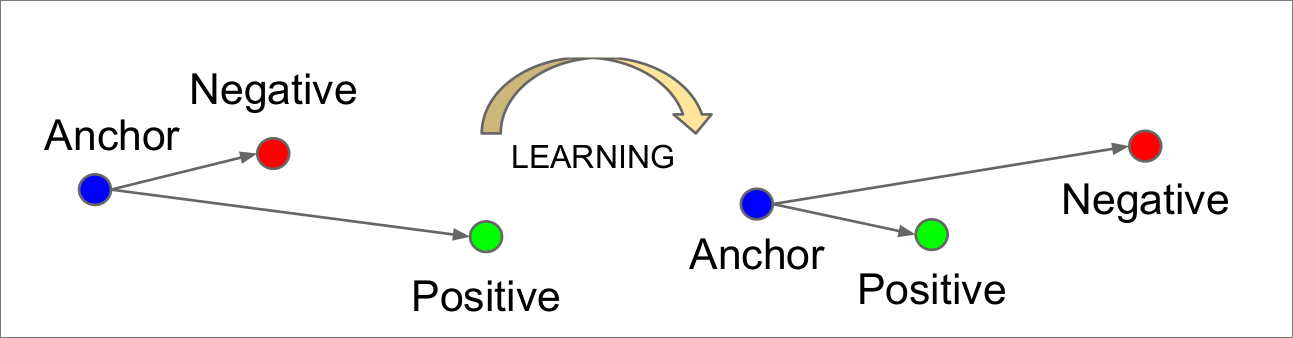
\includegraphics[width=0.8\textwidth]{informatica/triplet_loss_learning}
    \caption{Ejemplo gráfico del proceso de aprendizaje deseado con \textit{triplet loss}. Imagen extraída de \cite{informatica:facenet}}
\end{figure}

Sin embargo, en \eqref{ieq:triplet_loss_single_entry} trabajamos con una sola entrada de tres datos. A diferencia de un \textit{dataset} con datos etiquetados clásico (de la forma \lstinline{(entrada, valor de etiqueta)}), tenemos datos de la forma \lstinline{(imagen, identificador de individuo, edad)}. Esto supone un \textbf{problema} a resolver: cómo generamos \textit{batches} con triples de la forma \lstinline{(ancla, positivo, negativo)} para poder aplicar \eqref{ieq:triplet_loss_single_entry}. Introducimos algunas soluciones propuestas a este problema en \customref{isec:batching}

Por otro lado, este enfoque plantea algunas \textbf{ventajas}. La principal es que, a diferencia de otros enfoques basados en usar funciones de pérdida auxiliares (y que suelen fuerzan que la red solo pueda funcionar comparando pares de imágenes), el cómputo del \textit{embedding} es directo usando esta función de pérdida (\textit{end to end learning}). Optimizamos directamente la propiedad semántica del \textit{embedding} que deseamos obtener. Una vez entrenado el modelo es directo adaptar el modelo a tareas de \textit{clustering}, \textit{retrieval}, verificación, \ldots \cite{informatica:principal}

\section{Generación de \textit{batches}} \label{isec:batching}

Como ya hemos comentado, la tarea que debemos resolver ahora es la de generación de \textit{batches} adecuados para poder emplear \eqref{ieq:triplet_loss_single_entry} como función de pérdida a minimizar.

Por tanto, dado un conjunto de datos de la forma \lstinline{(imagen, identificador, edad)}, debemos obtener un conjunto de datos de la forma \lstinline{(img. ancla, img. positivo, img. negativo)}. Este último conjunto de datos puede ser una lista de triples o conjuntos de \textit{batches}. Como vamos a trabajar con \textit{batches}, podemos simplemente muestrear aleatoriamente y sin remplazo de la lista de triples, repitiendo el muestreo tras cada época completada.

\subsection{Enfoque \textit{offline}} \label{isubs:enfoque_offline_minado_triples}

Este es el enfoque clásico, que se ha venido usando previo a \cite{informatica:facenet}, que introduce un enfoque \textit{online} que luego otros trabajos como \cite{informatica:principal} han ido mejorando.

En este enfoque, el ciclo de aprendizaje se divide en \textbf{varios pasos}.

En primer lugar, se realiza un \textbf{minado \textit{offline}} de los triples. Es decir, se obtiene una primera lista (o conjunto de \textit{batches}) de la forma \lstinline{(img. ancla, img.positivo, img.negativo)}. Una forma de hacer esto sería, por ejemplo, generar los triples de forma aleatoria, generar todos los posibles triples, $\ldots\dspace$ Aunque estas ideas no suelen funcionar en la práctica. Otra forma más efectiva es seleccionar los triples en base de algún estudio estadístico. O usar la red que vamos a optimizar, para identificar aquellos triples en los que tiene más dificultad de distinguir.

En segundo lugar, realizamos el aprendizaje sobre dicho conjunto de triples. En algunos casos, realizamos el entrenamiento completo sobre dicho conjunto inicial. En otros casos, principalmente cuando usamos la red para el minado de triples, pasadas algunas épocas de entrenamiento volvemos a generar otra vez la lista de triples. Así, triples que antes la red no identificaba propiamente, ahora sí que los identifica (\entrecomillado{network snapshots}, \cite{informatica:facenet}) y podemos buscar triples más interesantes.

Una vez computado una lista de triples $(a, p, n) \in \Omega$, la función de pérdida \eqref{ieq:triplet_loss_single_entry} se implementa de forma natural como en cualquier otro ámbito de \textit{batching}:

\begin{equation}
    \mathcal{L}_{tri}^{offline}(\theta; \Omega) := \frac{1}{\#\Omega} \sum_{(a, p, n) \in \Omega} \mathcal{L}_{tri}(\theta; a, p, n)
\end{equation}

\begin{observacion}

Normalmente, en la literatura sobre aprendizaje automático, se ignora el término $\frac{1}{\#\Omega}$ y se supone que siempre estamos dividiendo por el número de sumandos, con lo que nuestra función de error suele escribirse como:

\begin{equation}
    \mathcal{L}_{tri}^{offline}(\theta; \Omega) := \sum_{(a, p, n) \in \Omega} \mathcal{L}_{tri}(\theta; a, p, n)
\end{equation}


\end{observacion}

Este enfoque supone una serie de \textbf{problemas}:

\begin{itemize}
    \item Estamos dividiendo el proceso de aprendizaje en dos etapas, la de minado de triples y la de aprendizaje sobre estos triples. Esto añade complejidad a nuestra \textit{pipeline}
    \item La adecuada elección de triples es fundamental. Si elegimos triples demasiado fáciles, la red no aprenderá nada nuevo, pues es muy fácil distinguir los ejemplos presentados. Sin embargo, si solo mostramos triples complicados, el modelo se centrará en aprender ejemplos extraordinarios y no sabrá distinguir el grueso de ejemplos más sencillos
        \begin{itemize}
            \item Además, generalmente los modelos aprenden rápidamente a distinguir la mayoría de ejemplos en los que las diferencias son relativamente evidentes. Por tanto, en pocas iteraciones la mayoría de triples son demasiado sencillos, lo que agrava mucho este problema
        \end{itemize}
    \item Lo ideal sería disponer de alguna forma de ajustar la complejidad de los triples presentados. Podemos confiar en que al ir re-generando la lista de triples, la complejidad vaya aumentando. Pero el algoritmo de minado debería tener alguna forma de controlar el énfasis que se hace en la búsqueda de combinaciones difíciles, lo que añade aún más complejidad al sistema
    \item El minado supone realizar un proceso de búsqueda, que es \textbf{muy lento} (evaluar de alguna forma todos los posibles triples supondría al menos $O(n^3)$). Lo ideal sería disponer de algún método que se basará en muestrear aleatoriamente de nuestra lista de \lstinline{(imagen, identidad, edad)} (proceso que es muy rápido) y generar rápidamente triples interesantes (esto es lo que hacemos en \customref{isubs:triples_online})
\end{itemize}

\subsection{Enfoque \textit{online}} \label{isubs:triples_online}

La idea común será implementar el siguiente proceso. En primer lugar, realizaremos un muestreo aleatorio sobre los datos de la forma \lstinline{(imagen, identidad, edad)}. Este muestreo es rápido y no supone prácticamente tiempo de cómputo. Usando únicamente los datos de ese muestreo, generaremos triples y computaremos la función de pérdida apoyándonos en \eqref{ieq:triplet_loss_single_entry}. Dicha generación ya sí que supone un tiempo de cómputo considerable. Repetimos este proceso hasta agotar todos las entradas de nuestro \textit{dataset}, completando así una época de entrenamiento.

Ya podemos ver algunas \textbf{ventajas de este método}, incluso antes de haber especificado las dos partes fundamentales (muestreo y selección de triples):

\begin{enumerate}
    \item La ventaja más obvia es que, suponiendo que el tamaño de la muestra es significativamente mucho más pequeño que el tamaño de todo el conjunto de datos, la generación de triples consumirá potencialmente menos tiempo y será más efectiva
        \begin{itemize}
            \item Para afirmar esto rotundamente, tendríamos que realizar un estudio del tiempo del minado \textit{offline} en contraste a la suma de todos los tiempos de minado en cada muestreo
            \item Sin embargo, el tiempo usado es más eficiente, porque en cada paso estamos usando la red actualizada. En el minado \textit{offline} podemos gastar muchísimo tiempo en encontrar triples difíciles que, tras entrenar en pocos ejemplos previos, acaben siendo sencillos, y por tanto, cuando la red vea estos ejemplos, ya sean totalmente inútiles
        \end{itemize}
    \item Se facilita en gran parte el ajuste de la dificultad. Podemos buscar triples realmente difíciles, pero como solo se tiene acceso a una pequeña muestra, estamos controlando la dificultad. Aquí podemos variar el tamaño de las muestras para buscar un punto medio entre ejemplos muy difíciles o ejemplos demasiado sencillos. Y todo esto sin contar con el factor de que vamos a usar la red actualizada para la elección de los triples, como comentaremos más adelante
\end{enumerate}

Desarrollada esta visión de forma general, veamos cómo se implementa cada una de las partes, siguiendo las técnicas introducidas en \cite{informatica:principal}.

\subsection{Muestreo de los datos con \textit{P-K sampling}}

La \textbf{idea principal del muestreo} es lo que definiremos como \textbf{\textit{P-K sampling}}. Como ya hemos comentado en \customref{isubs:triples_online}, nuestra tarea ahora es generar un \textit{batch} de elementos de la forma \lstinline{(imagen, identidad, edad)}. En una segunda etapa (véase \customref{isubs:seleccion_de_triples}), otro algoritmo decide como generar triples a partir de estos datos.

El algoritmo de muestreo \textit{P-K sampling} es muy sencillo. En cada muestreo, seleccionamos aleatoriamente $P$ identidades de individuos (o clases, en un ambiente más general en el que no necesariamente estemos trabajando con imágenes de personas). Por cada una de las identidades, seleccionamos aleatoriamente $K$ imágenes. Por tanto, obtenemos una lista de $P \cdot K$ imágenes, o lo que podemos llamar, un \textbf{\textit{P-K batch}}. Para poder obtener triples interesantes en la siguiente etapa, parece que lo deseable es que ambas selecciones aleatorias (muestreos) sean sin repetición.

El hecho de tener $K$ imágenes por cada uno de los individuos seleccionados es lo que va a permitir al algoritmo de generación de triples obtener rápidamente triples interesantes.

Queda aquí claro los problemas que introduce este muestreo: si queremos muestrear $K$ imágenes de cada individuo sin repetición, cada individuo debe tener asociadas al menos $K$ imágenes. Así que a la hora de trabajar con un \textit{dataset}, siempre deberíamos comprobar la distribución del número de imágenes por individuo, como hemos hecho en \customref{isec:base_datos_usada}.

\subsection{Selección de triples y funciones de pérdida} \label{isubs:seleccion_de_triples}

Una vez que tenemos un \textit{batch} de $P \cdot K$ elementos, deberemos seleccionar triples de ellos. Una vez se especifica cómo se seleccionan los triples, usando \eqref{ieq:triplet_loss_single_entry}, inducimos de forma natural y directa una cierta función de pérdida que actúa sobre estos \textit{P-K batches}.

\begin{observacion}

    Vamos a trabajar con $P \cdot K$ elementos, cada uno correspondiendo a una clase en concreto. Por tanto, indexaremos los elementos de la forma $x_k^p$ donde $p$ marca el identificador del individuo, y $k$ marca a cuál de las $K$ imágenes del individuo $p$ nos estamos refiriendo

\end{observacion}

\subsubsection{\textit{Batch Hard}} \label{isubsubs:batch_hard}

La primera idea es iterar sobre todos los elementos del \textit{P-K batch}, obteniendo así $P \cdot K$ anclas. Por cada ancla, seleccionamos el positivo y negativo \textbf{más complicado dentro de \textit{P-K batch}}. Por tanto, queda claro que \textbf{estamos usando la red para seleccionar triples difíciles} en cada \textit{batch} generado.

Esto introduce la siguiente función de pérdida, a la que llamaremos \textbf{\textit{Batch Hard}}:

\begin{equation}
    \mathcal{L}_{BH}(\theta, \hat{\Omega}) := \comentarencima{\sum_{p = 1}^P \sum_{k = 1}^K}{\text{todas las anclas}} [
        \comentarencima{\max_{k' = 1, \ldots, K} D(f_{\theta}(x_k^p), f_{\theta}(x_{k'}^p))}{\text{positivo más complicado}}
        - \comentarencima{\min_{\substack{p' = 1, \ldots, P \\ p' \neq p \\ k' = 1, \ldots, K}} D(f_{\theta}(x_k^p), f_{\theta}(x_{k'}^{p'}))}{\text{negativo más complicado}}
        + \alpha]_+
\end{equation}

donde $[x]_+ := max \{0, x\} = ReLU(x)$ y $\hat{\Omega}$ se refiere a un \textit{P-K batch}. No olvidemos que no estamos escribiendo la división por el número de sumandos, $P \cdot K$.

Estamos generando \textbf{triples moderados}, porque estamos buscando los triples más difíciles, pero dentro de un \textit{batch} relativamente pequeño comparado a el total del conjunto de datos. Por tanto, estamos ajustando la dificultad de los triples cómodamente, resolviendo el problema que comentábamos en \customref{isubs:enfoque_offline_minado_triples}. Aumentando el valor de $P, K$, aumentamos el espacio de búsqueda, y por tanto podremos encontrar triples mucho más difíciles. Sin embargo, hay que tener siempre en cuenta el coste en tiempo de cómputo.

Queda claro que, gracias al proceso de \textit{P-K sampling}, ahora es factible realizar una búsqueda de triples interesantes en profundidad, basándonos en el estado más actualizado de la red para calcular la dificultad de los triples. Esta búsqueda extensiva no habría sido posible si la planteásemos sobre todo el conjunto de datos.

\subsubsection{\textit{Batch All}} \label{isubsubs:batch_all}

Motivados por lo comentado en \customref{isubsubs:batch_hard}, podemos plantearnos usar todas los posibles triples dentro de un \textit{P-K batch} como un enfoque que ahora cobra más sentido (ya hemos comentado en \customref{isubs:enfoque_offline_minado_triples} que realizar esto sobre todo el conjunto de datos no parece una buena idea).

Realizar esto introduce la función de pérdida que llamaremos \textbf{\textit{Batch All}}:

\begin{equation} \label{ieq:batch_all}
    \mathcal{L}_{BA}(\theta; \hat{\Omega}) :=
    \comentarencima{\sum_{p = 1}^{P} \sum_{k = 1}^K}{\text{todas anclas}}
    \comentardebajo{\sum_{\substack{k' = 1 \\ k' \neq k}}^{K}}{\text{todas pos.}}
    \comentarencima{\sum_{\substack{p' = 1 \\ p' \neq p}}^P \sum_{n = 1}^K}{\text{todas neg.}} \dspace[
        D(f_{\theta}(x_k^p),f_{\theta}(x_{k'}^p)) - D(f_{\theta}(x_k^p),f_{\theta}(x_{n}^{p'})) + \alpha
    ]_+
\end{equation}

Está claro que, por el número de sumandos, esta aproximación es viable gracias a que nuestro \textit{P-K sampling} reduce mucho el número de elementos sobre los que operamos. Dicho número de sumandos viene dado por:

\begin{equation}
    P \cdot K \cdot (K - 1) \cdot (P - 1) \cdot K = P^2 - P + K^3 - K^2 \approx P^2 + K^3
\end{equation}

Esta aproximación sería completamente inviable sobre un número muy elevado de elementos. Pensemos, por ejemplo, en las 163446 imágenes de \textit{CACD}.

\subsubsection{Mejoras introducidas a partir de la experimentación}

En \cite{informatica:principal}, a raíz de observar los resultados de la experimentación, señalan algunos puntos débiles en las dos funciones de pérdida que introducen a partir del \textit{P-K sampling}.

Principalmente, en \customref{isubsubs:batch_all}, podemos ver un posible fallo en la función de pérdida \eqref{ieq:batch_all}. Si se da el caso de que la mayoría de triples generados son fáciles (hecho muy probable al estar generando todas las combinaciones de triples), los escasos triples que realmente son difíciles se desvanecerán. Esto porque la mayoría de términos serán cero (al estar aplicando $[x]_+$). Y los pocos términos que no son cero, se dividen por el número total de elementos, que ya hemos visto que es elevado.

Por tanto, una mejora sencilla a esta función de pérdida es dividir únicamente por el número de sumandos no nulos. Esta mejora la podemos aplicar también a \textit{batch hard}, obteniendo dos nuevas funciones de pérdida, a las que llamaremos $\mathcal{L}_{BA \neq 0}$ y $\mathcal{L}_{BH \neq 0}$.

\subsubsection{Algunas observaciones y conclusiones}

En primer lugar, cabe destacar que, como señalan \cite{informatica:principal}, las dos nuevas funciones de pérdida introducidas equivalen al planteamiento clásico de \textit{triplet loss} si entrenásemos indefinidamente.

El desarrollo que hemos realizado justifica las siguientes \textbf{ventajas} de los nuevos métodos:

\begin{itemize}
    \item El uso del \textit{P-K sampling} y las dos nuevas funciones de pérdida (con las variantes técnicas) permiten realizar el aprendizaje de forma usual, sin añadir un paso adicional en el bucle de aprendizaje, evitando así la gran complejidad añadida del minado \textit{offline}
    \item Además, conseguimos un manejo preciso de la dificultad de los triples obtenidos. Controlando el valor de $\{P, K\}$, controlamos el espacio de búsqueda y, en definitiva, la dificultad. Todo esto de forma cómoda y sin introducir apenas complejidad en nuestro \textit{pipeline}
    \item Aunque no lo hemos comprobado, pensamos que esto acelera los tiempos de cómputo, al estar realizando el minado de triples sobre \textit{batches} de tamaño considerablemente reducidos
    \item Y aunque no mejorásemos el tiempo de computo, lo que sí sabemos que mejoramos es la eficacia del minado de triples. El minado de triples usa una red mucho más actualizada, para generar una lista mucho más pequeña que probablemente no se degrade tanto como la generada por un minado \textit{offline} sobre todo el conjunto de datos, mucho más grande
    \item Es más, estamos controlando el efecto de los triples demasiado sencillos, que no tendremos en cuenta a la hora de dividir los sumandos en la función de pérdida
\end{itemize}

A pesar de esto, a raíz de trabajar con estas nuevas técnicas, identificamos los siguientes \textbf{inconvenientes}:

\begin{itemize}
    \item Introducimos dos hiperparámetros, $\{P, K\}$, que deberemos ajustar correctamente, pues tienen un enorme impacto en los resultados del proceso de entrenamiento. Por tanto, se hace fundamental tener un proceso de \textit{hyperparameter tuning} robusto, como introducimos en \customref{isec:hp_tuning}
    \item Tenemos que tener mucho cuidado con valores elevados de $\{P, K\}$, por dos motivos. El primero, y como ya hemos comentado, valores altos implicarán que los tiempos de cómputo para la generación de triples crecerán rápidamente. El segundo es que el tamaño de los \textit{batches} crecerán considerablemente, llegando a colapsar la memoria disponible de la \textit{GPU}
    \item Hemos comprobado en la práctica que es realmente fácil colapsar la memoria \textit{GPU}, usando modelos profundos como \textit{ResNet50} con valores de $P \cdot K > 200$. Esto supone que, aunque no estuviéramos limitados por el tiempo de cómputo, el colapso de la memoria limita el conjunto de valores que $\{P, K\}$ puede tomar, restringiendo fundamentalmente la experimentación que podemos realizar con estos valores
    \item Si queremos usar valores altos de $K$, nuestro \textit{dataset} lo debe permitir, teniendo una buena distribución de imágenes por individuo (por esto, hemos realizado este estudio en \customref{isec:base_datos_usada} para nuestras bases de datos). Se pueden explorar técnicas como el aumentado de datos para aumentar el número de imágenes por individuo, pero solo serán efectivas si dicha distribución es buena para empezar
    \item Tanto por el formato de los datos con los que hemos trabajado, como por el cambio fundamental realizado en el \textit{sampling} de los datos, hemos tenido que realizar un \textbf{esfuerzo considerable de implementación}, al no poder basarnos en la mayor parte de los casos en código implementado por alguna biblioteca de aprendizaje automático. Esto se ve reflejado en \customref{ich:implementacion}
\end{itemize}

\section{Función de distancia}


\section{Métricas}

\todo{Hablar de rank@k, distancias intracluster, intercluster, silhouette, ...}

\section{Hablar de la tarea de retrieval?}

\chapter{Modelización de la tarea de aprendizaje} \label{ch:tarea_aprendizaje}

\section{Planteamiento del problema} \label{seq:planteamiento_problema}

La tarea de aprendizaje que consideramos es la de \textbf{clasificación de imágenes}, para la cual el uso de redes convolucionales profundas ha supuesto un gran avance. Nos centraremos en modelar redes convolucionales (profundas y no profundas) para clasificar imágenes.

Dado un elemento $X = (\nv{x_1}, \ldots, \nv{x_N})$, donde $\nv{x_i} \in \R^s \ \forall i \in \deltaset{N}$, queremos clasificarlo en alguna de las etiquetas $\mathcal{Y} = \{1, \ldots, Y \} = \deltaset{Y}$. Con esto, podemos ver que los datos de entrada viven en el espacio

\begin{equation}
	\mathcal{X} := \R^s \times \overset{N}{\ldots} \times \R^s = (\R^s)^N.
\end{equation}

Esta representación de los datos de entrada es natural en muchos escenarios. En el caso de las imágenes, podemos considerar cada vector $\nv{x_i}$ como un conjunto de \textit{pixels} de la imagen, en lo que se conoce como parche o \textit{patch}. Por la estructura local de las imágenes, cada parche debería contener un vecindario de \textit{pixels}, es decir, \textit{pixels} adyacentes. Puede ocurrir que los parches no sean disjuntos, o lo que es lo mismo, que existan \textit{pixels} perteneciendo a más de un parche. Las imágenes contienen información en los colores que contiene cada píxel, pero también en su posición. Esto es claro si tenemos en cuenta que permutando aleatoriamente las posiciones de los \textit{pixels} de una imagen, ésta pierde el sentido. Mostramos un ejemplo de ello en la \imgref{img:desordenar_pixeles_repetida_mates}. A esto nos referimos cuando hablamos de estructura local de la imagen. Una forma natural de generar estos parches a partir de las imágenes consiste en tomar $\nv{x_i}$ como la fila o columna $i$-ésima de la imagen.

\begin{figure}[!hbtp]
	\centering
	\ajustarsubcaptions
	\begin{subfigure}[t]{0.45\textwidth}
		\centering
		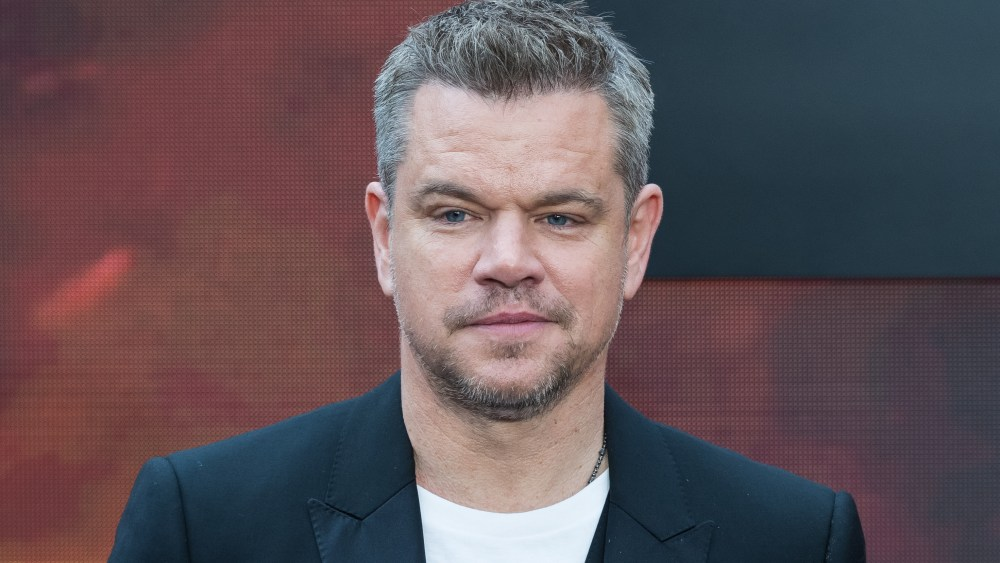
\includegraphics[width=0.9\linewidth]{informatica/ejemploperm_normal}
		\caption{Imagen original}
	\end{subfigure}
	\begin{subfigure}[t]{0.45\textwidth}
		\centering
		
\includegraphics[width=0.9\linewidth]{informatica/ejemploperm_permutada}
		\caption{Imagen original tras aplicar una permutación aleatoria de las posiciones de los \textit{pixels}}
	\end{subfigure}
	\caption{Tenemos que considerar la estructura local de la imagen. La posición de los \textit{pixels} y su vecindario contiene una información fundamental de la que no podemos prescindir. Por tanto, los parches deben contener vecindarios de \textit{pixels}, aunque tengamos distintas estrategias para escoger estos vecindarios.}
	\label{img:desordenar_pixeles_repetida_mates}
\end{figure}

Para decidir la etiqueta de un elemento, consideramos $Y$ \textbf{funciones de puntuación}:

\begin{equation}
	\conjunto{h_y: \mathcal{X} \to \R \dspace / \dspace y \in \mathcal{Y}}.
\end{equation}

\textbf{NOTA PARA JAVIER}: aquí me marcaste debajo de $Y$ y de $\mathcal{Y}$. Escribo $Y$ funciones de puntuación y luego $y \in \mathcal{Y}$ porque he definido $\mathcal{Y} := \deltaset{Y}$. No sé si esta definición aporta poco y lía más que otra cosa, en cuyo caso creo que es mejor quitar la definición de $\mathcal{Y} := \deltaset{Y}$. O si simplemente crees que es mejor que escoja una tipografía o letras que líen menos.
\todo{Borrar esta nota para Javier}

Con esto, dado un elemento $X \in \mathcal{X}$, lo clasificaremos buscando la etiqueta cuya función de puntuación sea máxima, es decir:

$$\hat{y} := \underset{y \in \mathcal{Y}}{argmax} \dspace h_y(X).$$

Por tanto, nuestro \textbf{espacio de hipótesis} es el conjunto de funciones $\Gamma := \conjunto{f: \mathcal{X} \to \R}$. Tanto en la práctica con modelos reales de aprendizaje automático como en nuestras dos modelizaciones, trabajamos en un subconjunto $\tilde{\Gamma} \subseteq \Gamma$ de funciones de puntuación, implementables o bien por el modelo de \textit{machine learning} o bien por nuestra modelización teórica.

\section{Espacio de hipótesis general} \label{sec:espacio_hipotesis_general}
\todo{JMERI: leer de nuevo esta sección completa, porque es muy liosa, repito cosas, introduzco cosas donde no debería. Mirar los contenidos que he borrado}

Nuestro objetivo en esta sección es justificar la elección de las funciones $h_y$ que conformarán el espacio de hipótesis sobre el que trabajaremos. En la \sectionref{sec:repr_funciones_puntuacion} mostramos cuál es la elección final basada en el desarrollo previo. Usaremos ciertos hechos básicos sobre análisis funcional que hemos introducido en la \sectionref{sec:preliminares_funcional}.

\subsection{Planteamiento para construir el espacio de hipótesis} \label{sec:justificacion_func_repr}

Recordemos que los datos de entrada viven en el espacio $\mathcal{X} = (\R^s)^N$ y que, para cada entrada $X \in \mathcal{X}$, tomamos como salida la etiqueta $\hat{y} \in \mathcal{Y}$ que maximice su función de puntuación asociada, que venía dada como:

\begin{equation}
	\hat{y} := \underset{y \in \mathcal{Y}}{argmax} \dspace h_y(X).
\end{equation}

Por lo tanto, buscamos \textbf{construir un espacio de hipótesis} $\mathcal{H} \subseteq L^2((R^s)^N)$ donde elegir nuestras funciones de puntuación. Dicha elección influirá en los modelos de aprendizaje que podamos desarrollar.

Comenzaremos tomando un conjunto de funciones $\conjunto{f_d(\nv{x}): \; d \in \N} \subseteq L^2(\R^S)$ de forma que sea total y linealmente independiente. Llamaremos \textbf{funciones de representación} a las funciones de este conjunto. Gracias a la \propref{prop:conservacion_totalidad_indp_lineal_func_prod} sabemos que la familia de funciones producto inducida $\conjunto{(\nv{x_1}, \ldots, \nv{x_n}) \mapsto \prod_{i = 1}^N f_{d_i}(\nv{x_i}) }_{d_1, \ldots, d_N \in \N} \subseteq L^2((\R^S)^N)$ es también total y linealmente independiente. Por ser total, la \propref{prop:conjuntos_totales_epsilon_aproximacion} nos dice que podemos aproximar funciones de $L^2((\R^S)^N)$ arbitrariamente bien con combinaciones lineales finitas de funciones producto. En la \sectionref{sec:funciones_representacion} hemos visto que podemos escoger funciones de base radial \textit{RBF} o neuronas para tomar un conjunto de funciones de representación que sea total, linealmente independiente y además finito.
\todo{JMeri: hacer la prueba de estos dos resultados que menciono, porque mi desarrollo matemático depende de ellos}

\subsection{Representación tensorial}

Con todo lo anterior tenemos $\epsilon$-aproximación a partir de combinaciones lineales finitas de elementos de un conjunto infinito. Vamos a representar esta aproximación con tensores, lo que nos permitirá más tarde trabajar con modelizaciones basadas en descomposiciones tensoriales. Para ello, consideraremos tensores formales $\mathcal{A}^y \in \espaciotensores{N}{\N}$. Esto es, tensores con $N$ modos, cada modo con una dimensión infinita numerable (podemos considerar que tenemos $N$ sucesiones). El papel de estos tensores formales será el de almacenar los coeficientes de la combinación lineal finita dada por la ecuación \eqref{eq:conjuntos_totales_epsilon_aproximacion} y, por lo tanto, los llamaremos \textbf{tensores de coeficientes}. Como esa combinación lineal es finita, nuestro tensor formal tendrá todas las entradas nulas salvo un conjunto finito. Necesitamos usar tensores formales porque tenemos que elegir qué funciones usamos de un conjunto numerable. Y con esto llegamos a:

\begin{equation} \label{eq:hipotesis_en_general}
	h_y(\nv{x_1}, \ldots, \nv{x_N}) \approx \sum_{d_1, \ldots, d_N \in \N} A^y_{d_1, \ldots, d_N} \prod_{i = 1}^N f_{d_i}(\nv{x_i}).
\end{equation}

Como hemos visto que podemos tomar un conjunto de funciones de representación total, linealmente independiente y además finito, es suficiente considerar $\mathcal{A}^y \in \espaciotensores{N}{M}$ para algún $M \in \N$, con lo que el modelo queda:

\begin{equation}
	h_y(\nv{x_1}, \ldots, \nv{x_N}) \approx \sum_{d_1, \ldots, d_N = 1}^{M} \mathcal{A}^y_{d_1, \ldots, d_N} \prod_{i = 1}^N f_{\theta_{d_i}}(\nv{x_i}).
\end{equation}

De esta forma, este modelo será universal. Podemos aproximar arbitrariamente bien cualquier función de puntuación $h_y \in L^2((\R^S)^N)$ con combinaciones lineales, expresadas a partir de la ecuación anterior. Además, como el conjunto de funciones es linealmente independiente, la expresión anterior es única, y nuestro conjunto de funciones actúa de base del espacio. Es decir, una función de puntuación $h_y$ determina únivocamente el tensor de coeficientes $\mathcal{A}^y$, y podemos escribir:

\begin{equation} \label{eq:puntuacion_general}
	h_y(\nv{x_1}, \ldots, \nv{x_N}) = \sum_{d_1, \ldots, d_N = 1}^{M} \mathcal{A}^y_{d_1, \ldots, d_N} \prod_{i = 1}^N f_{\theta_{d_i}}(\nv{x_i}).
\end{equation}

Así, la tarea de aprendizaje consistirá en aprender a partir de los datos de entrenamiento los coeficientes $\theta_1, \ldots, \theta_M$ de las funciones de representación y los tensores de coeficientes $\mathcal{A}^1, \ldots, \mathcal{A}^Y$.

\begin{observacion}
	Usamos la notación $\sum_{d_1, \ldots, d_N = 1}^{M}$ para denotar $\sum_{d_1 = 1}^{M} \sum_{d_2 = 1}^{M} \ldots \sum_{d_N = 1}^{M}$.
\end{observacion}

\subsection{Capa de representación} \label{subs:capa_de_representacion}

En la ecuación \eqref{eq:puntuacion_general} estamos usando las mismas funciones de representación $f_{\theta_1}, \ldots, f_{\theta_M}: \R^s \to \R$ para todas las funciones de puntuación $h_y$. Lo único que cambia entre las distintas funciones de puntuación es el tensor de coeficientes $\mathcal{A}^y$. Nótese además que en la ecuación \refeq{eq:puntuacion_general}, los vectores de entrada $\nv{x_i}$ solo participan en el producto que involucra computar $f_{\theta_{d_i}}(\nv{x_i})$. Por tanto, podemos considerar un paso inicial, que será compartido en los dos modelos que más adelante introduciremos, consistente en computar los valores:

$$\{f_{\theta_d}(\nv{x_i}): \; d \in \deltaset{M},\ i \in \deltaset{N} \}.$$

Una vez que hayamos computado esos $M \cdot N$ valores, ya no necesitamos los vectores $\nv{x_i}$ para nada más. Con esto, es natural considerar que nuestro modelo tenga una primera capa que compute esos valores, a la que llamaremos \textbf{capa de presentación} y que será una capa convolucional con $M$ canales. Por tanto, cada parche de entrada $\nv{x_i} \in \R^s$ acaba siendo representando por un descriptor de longitud $M$. Con esto, en todas las funciones de puntuación los descriptores resultado de la capa de representación serán los mismos. El siguiente diagrama muestra gráficamente cómo actúa la capa de representación, calculando los $N \cdot M$ coeficientes reales que componen los descriptores de dicha capa:

\begin{figure}[!hbtp]
	\centering
	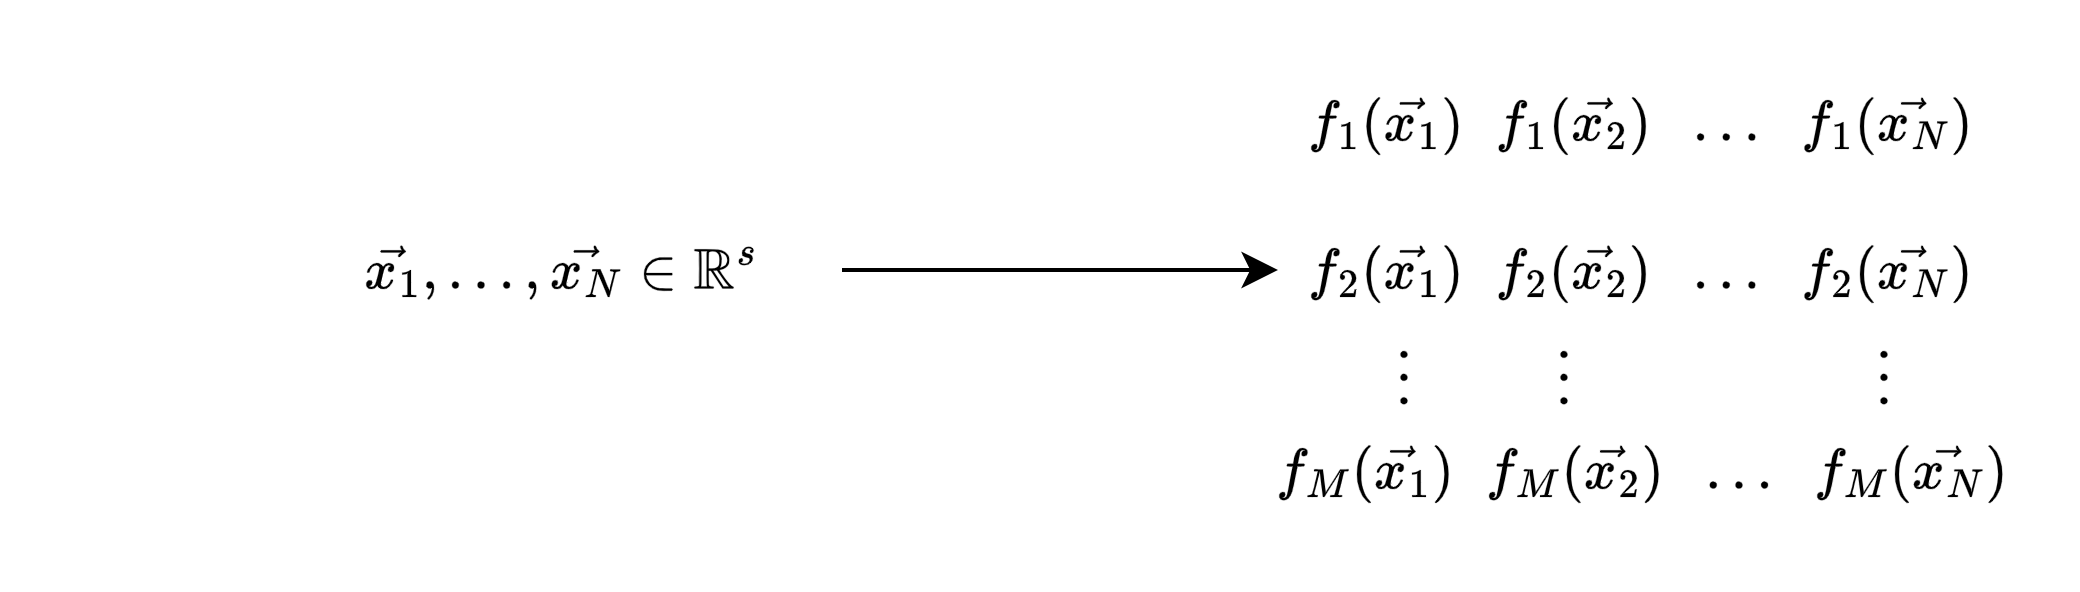
\includegraphics[width=0.8\textwidth]{matematicas/computo_capa_representacion}
	\caption{Ejemplo gráfico sobre cómo actúa la capa de representación. A partir de $N$ parches en $\R^s$, acabamos con $N \cdot M$ coeficientes reales que conformen los descriptores de la capa.}
\end{figure}


\subsection{Ejemplo de cómputo} \label{ejemplo:funcion_puntuacion}

Supongamos que trabajamos con $N = 3, M = 2$. En este caso, una imagen de entrada se compone de los vectores $\nv{x_1}, \nv{x_2}, \nv{x_3} \in \R^s$ (no estamos interesados en el valor de $s \in \N$). Y tenemos dos funciones de representación $f_1, f_2: \R^s \to \R$. El primer paso es computar la capa de representación, que son los $N \cdot M$ coeficientes reales dados por:

\begin{equation}
	\begin{split}
		f_1(\nv{x_1}), f_1(\nv{x_2}), f_1(\nv{x_3}) \\
		f_2(\nv{x_1}), f_2(\nv{x_2}), f_2(\nv{x_3})
	\end{split}
\end{equation}

Y con esto ya podemos expresar nuestra función de puntuación:

\begin{equation}
	\begin{split}
		h_y(\nv{x_1}, \ldots, \nv{x_N}) &= \sum_{d_1, d_2, d_3 = 1}^{2} \mathcal{A}^y_{d_1 d_2 d_3} \prod_{i = 1}^3 f_{d_i}(\nv{x_i}) = A_{111} \; f_1(\nv{x_1}) \; f_1(\nv{x_2}) \; f_1(\nv{x_2}) + A_{112} \; f_1(\nv{x_1}) \; f_1(\nv{x_2}) \; f_2(\nv{x_2}) + \\
		\cdots &+ A_{321} \; f_3(\nv{x_1}) \; f_2(\nv{x_2}) \; f_1(\nv{x_2}) + A_{333} \; f_3(\nv{x_1}) \; f_3(\nv{x_2}) \; f_3(\nv{x_3}).
	\end{split}
\end{equation}

Queda claro que el tensor $\mathcal{A}^y$ contiene los coeficientes que realizan una combinación lineal sobre todos los posibles productos de nuestros $N \cdot M$ valores reales de la capa de representación.

\section{Resumen}

Buscamos resolver una tarea de clasificación de imágenes. Dada una imagen de entrada, debemos asignarle una de las etiquetas $\mathcal{Y} := \{1, \ldots, Y\} = \deltaset{Y}$. Para ello, tomamos la etiqueta cuya función de puntuación asociada $h_y$ sea mayor. Las imágenes de entrada se dividen en parches. Esto es, una imagen viene dada por $N$ vectores $x = (\nv{x_1}, \ldots, \nv{x_N}), \dspace \nv{x_i} \in \R^s \dspace \forall i \in \deltaset{N}$. Elegimos un conjunto finito de funciones de representación que sea total y linealmente independiente. Para ello podemos elegir funciones de base radial \textit{RBF} o neuronas. Aplicando adecuadamente las propiedades del conjunto de funciones, llegamos a la modelización:

\begin{equation}
	h_y(\nv{x_1}, \ldots, \nv{x_N}) = \sum_{d_1, \ldots, d_N = 1}^{M} \mathcal{A}^y_{d_1, \ldots, d_N} \prod_{i = 1}^N f_{\theta_{d_i}}(\nv{x_i}).
\end{equation}

Estudiando esta ecuación nos damos cuenta de que hay un cómputo compartido en todas las funciones de puntuación, que encapsulamos en la capa de representación. Lógicamente, el cómputo de esta capa es compartido para todas las funciones de puntuación.

Las dos arquitecturas que introduciremos más adelante son el resultado de factorizar el tensor de coeficientes $\mathcal{A}^y$ con distintas descomposiciones. Ambas incorporan conceptos claves en la práctica del aprendizaje automático, como la localidad, coeficientes compartidos y \textit{pooling}.

\chapter{Modelización de las redes neuronales} \label{ch:modelizacion}

A partir de las herramientas matemáticas que hemos introducido en \customref{ch:matematicas_fundamentales} y de la modelización de la tarea de aprendizaje realizada en \customref{ch:tarea_aprendizaje}, buscamos desarrollar una modelización matemática de las redes neuronales con las que se suele trabajar en la práctica. Para que sea una \textbf{buena modelización}, esta debería cumplir que:

\begin{itemize}
    \item Sea lo más parecida a los modelos que se usan en la práctica
    \item Permita obtener resultados interesantes
\end{itemize}

Usando descomposiciones tensoriales, modelaremos dos tipos de redes:

\begin{itemize}
    \item Redes neuronales no profundas, a partir
    \todo{no se que nombre le dan a cada una de las redes en el paper!}
    \item Redes convolucionales profundas, a partir de los \textit{circuitos convolucionales aritméticos}
\end{itemize}

Creemos que la \textbf{modelización es muy cercana a las redes usadas en la práctica}. Principalmente, porque tiene en cuenta las tres propiedades características de una red convolucional:

\begin{enumerate}
    \item Localidad
    \item Compartición de parámetros, que junto a la localidad, da lugar a la convolución
    \item \textit{Pooling}
\end{enumerate}
\todo{Esto ya lo digo antes en la introducción. No sé si aquí sería buen momento para desarrollar lo que significa cada cosa o si es mejor quitarlo de alguna parte}

Además, los \textit{circuitos convolucionales aritméticos} son equivalentes a las redes conocidas como \textit{SimNets}, lo que reafirma el hecho de que la modelización es muy buena.
\todo{Esta afirmación la tendría que justificar, aunque sea referenciando al paper principal}

\section{Modelo CP}

Como ya hemos comentado en \customref{sec:repr_funciones_puntuacion}, buscaremos descomponer el tensor de coeficientes $\mathcal{A}^y$ que aparece en la ecuación \eqref{eq:puntuacion_general}, para que el aprendizaje de sus coeficientes sea computacionalmente factible.

La idea más simple es aplicar la \textit{descomposición CP}, que introducimos en \eqref{eq:cp_decomp}, en la ecuación \eqref{eq:puntuacion_general}. Usaremos una descomposición conjunta para los tensores:

\begin{equation} \label{eq:cp_decomp_conjunta}
    \mathcal{A}^y = \sum_{z = 1}^Z a_z^y \cdot \nv{\omega^{z, 1}} \otimes \ldots \otimes \nv{\omega^{z, N}}
\end{equation}

\todo{En la ecuación que introduzco antes no tengo escalares en la sumatoria!}

Desarrollemos los elementos que participan en esa ecuación. En primer lugar, sabemos por \eqref{eq:cp_decomp} que $a_z^y \in \R$, y por tanto, podemos considerar $\nv{a^y} := (a_1^y, \ldots, a_Z^y)^T \in \R^Z$. En segundo lugar, y de nuevo, conforme a \eqref{eq:cp_decomp}, tenemos los vectores $\nv{\omega^{z, i}} \in \R^M$ con $z \in \deltaset{Z}$, $i \in \deltaset{N}$. Decimos que la \textbf{descomposición es conjunta} porque los vectores $\nv{\omega^{z, i}}$ son los mismos para todos los valores de $y \in \mathcal{Y}$. Solo cambian los coeficientes $\nv{a^y}$, como bien refleja la elección de índices de la fórmula.

\begin{proposicion}
    Tomando $Z = M^N$ en la ecuación \refeq{eq:cp_decomp_conjunta}, la descomposición es universal. Esto es, podemos fijar un conjunto de vectores $\{\nv{\omega^{z, i}} \in \R^M / z \in \deltaset{Z}, i \in \deltaset{N} \}$ de forma que cualquier tensor $\mathcal{A}^y$ de orden $N$ y dimensión $M$ en cada modo puede ser representado. Es decir:

    \begin{equation}
        \forall \mathcal{A}^y \in \espaciotensores{N}{M}, \exists \nv{a^y} \in \R^Z: \text{la ecuación \refeq{eq:cp_decomp_conjunta} se verifica}
    \end{equation}
\end{proposicion}

\begin{proof}
    La idea de la demostración es muy sencilla. Tenemos que expresar un tensor arbitrario $\mathcal{A}$ de orden $N$ y dimensión $M$ en cada modo (es decir, de $M^N$ elementos) como una suma de $M^N$ elementos. Por tanto, en cada sumando, buscamos generar un único elemento del tensor y colocarlo en los índices apropiados. Es decir, cada sumando será un tensor de todo ceros salvo la entrada de la que nos ocupamos en esa iteración.

    Para que la demostración sea más clara cambiaremos la forma de indexar la suma. En la proposición estamos usando un único índice que llega hasta $Z = M^N$. Esto es lo mismo que usar $N$ índices que lleguen hasta $M$, y así la sumatoria queda:

    \begin{equation}
        \mathcal{A} = \sum_{i_1 = 1, \ldots, i_N = 1}^M a_{(i_1, \ldots, i_N)} \cdot \nv{\omega^{(i_1, \ldots, i_N), 1}} \otimes \ldots \otimes \nv{\omega^{(i_1, \ldots, i_N), N}}
    \end{equation}

    Para llevar a cabo la idea de usar cada sumando para colocar un elemento de $\mathcal{A}$ en sus índices correctos, haremos que en cada sumando se verifique

    \begin{itemize}
        \item $a_{i_1, \ldots, i_N} = \mathcal{A}_{i_1, \ldots, i_N}$. Esto es inmediato y no necesita más explicación
        \item $\nv{\omega^{(i_1, \ldots, i_N), 1}} \otimes \ldots \otimes \nv{\omega^{(i_1, \ldots, i_N), N}}$ genere el tensor en $\espaciotensores{N}{M}$ que sea cero en todas las entradas salvo en el índice $(i_1, \ldots, i_N)$, donde valdrá 1. Dicho tensor lo podemos denotar como  $\mathcal{B}^{(i_1, \ldots, i_N)}$
    \end{itemize}

    Ahora, veamos cómo podemos generar el tensor $\mathcal{B}^{(i_1, \ldots, i_N)}$ como producto tensorial de ciertos vectores. La propiedad fundamental que queremos que ese tensor cumpla es:

    \begin{equation}
        \mathcal{B}^{(i_1, \ldots, i_N)}_{j_1, \ldots, j_N} =
        \begin{cases}
            1 & \text{si } i_1 = j_1, \ldots, i_N = j_N \\
            0 & \text{en otro caso}
        \end{cases}
    \end{equation}

    Definimos $\nv{\delta_{i, N}}$ como el vector de longitud $N$, con todas las entradas nulas salvo la entrada de la posición $i$, en la que ponemos un uno. Por tanto, es claro que:

    \begin{equation}
        (\nv{\delta_{i, N}})_k =  \delta_{i, k}
    \end{equation}

    Definimos

    \begin{equation}
        \mathcal{B}^{(i_1, \ldots, i_N)} := \nv{\delta_{i_1, N}} \otimes \ldots \otimes \nv{\delta_{i_N, N}}
    \end{equation}

    y por tanto se verifica que:

    \begin{equation}
        \mathcal{B}^{(i_1, \ldots, i_N)}_{j_1, \ldots, j_N} = (\vec{\delta}_{i_1, N})_{j_1} \cdot \ldots \cdot (\vec{\delta}_{i_N, N})_{j_N} = \delta_{i_1, j_1} \cdot \ldots \cdot \delta_{i_N, j_N} =
        \begin{cases}
            1 & \text{si } i_1 = j_1, \ldots, i_N = j_N \\
            0 & \text{en otro caso}
        \end{cases}
    \end{equation}

    como buscábamos. Para concluir la demostración, fijamos el conjunto de vectores de forma que:

    \begin{equation} \label{eq:cp_decomp_asignacion_vectores}
        \{\nv{\omega^{z, i}} \in \R^M / z \in \deltaset{Z}, i \in \deltaset{N} \} =
        \{ \nv{\delta_{i_j, N}} / j \in \deltaset{N}, i_j \in \deltaset{M} \}
    \end{equation}

\end{proof}

\begin{observacion}
    En \eqref{eq:cp_decomp_asignacion_vectores} vemos que estamos usando menos vectores que los que se consideran en el enunciado del teorema. Esto es porque estamos repitiendo estos vectores. Por ejemplo, todos los sumandos referentes al valor 1 del primer índice tiene como primer vector $\vec{\delta}_{1, N}$
\end{observacion}

\begin{observacion}
    Esta proposición nos sirve para tener una cota superior del número de sumandos necesarios para realizar la descomposición. No hemos ganado nada respecto al trabajo previo. Seguimos teniendo el problema de considerar $M^N$ elementos, problema que ya vimos en \customref{sec:justificacion_func_repr}
\end{observacion}

Veamos ahora cómo podemos aplicar esta descomposición conjunta en nuestra ecuación \customref{eq:puntuacion_general}. Partimos de las dos ecuaciones:

\begin{equation}
\begin{split}
    h_y(\nv{x_1}, \ldots, \nv{x_N}) &= \sum_{d_1, \ldots, d_N = 1}^{M} \mathcal{A}^y_{d_1, \ldots, d_N} \prod_{i = 1}^N f_{\theta_{d_i}}(\nv{x_i}) \\
    \mathcal{A}^y &= \sum_{z = 1}^Z a_z^y \cdot \nv{\omega^{z, 1}} \otimes \ldots \otimes \nv{\omega^{z, N}} \\
\end{split}
\end{equation}

Ahora, sustituimos la segunda ecuación en la primera:

\begin{equation}
\begin{split}
    h_y(\nv{x_1}, \ldots, \nv{x_N}) &= \sum_{d_1, \ldots, d_N = 1}^{M} (\sum_{z = 1}^Z a_z^y \cdot \nv{\omega^{z, 1}} \otimes \ldots \otimes \nv{\omega^{z, N}}) \prod_{i = 1}^N f_{\theta_{d_i}}(\nv{x_i}) = \ldots \\
    \ldots &=  \sum_{z = 1}^Z \dspace \sum_{d_1, \ldots, d_N = 1}^{M} a_z^y \cdot \nv{\omega^{z, 1}} \otimes \ldots \otimes \nv{\omega^{z, N}} \prod_{i = 1}^N f_{\theta_{d_i}}(\nv{x_i}) = \ldots \\
    \ldots &=  \sum_{z = 1}^Z a_z^y \sum_{d_1, \ldots, d_N = 1}^{M} \nv{\omega^{z, 1}} \otimes \ldots \otimes \nv{\omega^{z, N}} \prod_{i = 1}^N f_{\theta_{d_i}}(\nv{x_i}) = \ldots \\
    \ldots &=  \sum_{z = 1}^Z a_z^y \sum_{d_1, \ldots, d_N = 1}^{M} \dspace \prod_{i = 1}^N \nv{\omega^{z, 1}} \otimes \ldots \otimes \nv{\omega^{z, N}} \cdot f_{\theta_{d_i}}(\nv{x_i}) = \ldots \\
    \ldots &=  \sum_{z = 1}^Z a_z^y \dspace \prod_{i = 1}^N \dspace \sum_{d_1, \ldots, d_N = 1}^{M}  \nv{\omega^{z, 1}} \otimes \ldots \otimes \nv{\omega^{z, N}} \cdot f_{\theta_{d_i}}(\nv{x_i}) = \ldots \\
    \ldots &=  \sum_{z = 1}^Z a_z^y \dspace \prod_{i = 1}^N \dspace \sum_{d = 1}^{M} \omega^{z, i}_d \cdot f_{\theta_{d}}(\nv{x_i})
\end{split}
\end{equation}
\todo{Tengo que desarrollar en papel bien este desarrollo que no tengo nada claro. El último paso no lo tengo controlado. Es la eq. (3) del paper de referencia}

Por lo tanto, nuestro \textbf{Modelo CP} se puede describir con la ecuación:

\begin{equation} \label{eq:cp_model}
    h_y(\nv{x_1}, \ldots, \nv{x_N}) =  \sum_{z = 1}^Z a_z^y \dspace \prod_{i = 1}^N \dspace \sum_{d = 1}^{M} \omega^{z, i}_d \cdot f_{\theta_{d}}(\nv{x_i})
\end{equation}

Veamos cómo esta ecuación se relaciona con un modelo usual de \textit{machine learning}. En primer lugar, y como ya hemos comentado en \customref{sec:repr_funciones_puntuacion}, el primer paso de nuestro modelo puede considerarse computar la capa de representación, esto es, los valores

$$\{f_{\theta_d}(\nv{x_i}) / d \in \deltaset{M},\ i \in \deltaset{N} \}$$

Una vez hecho esto, en \eqref{eq:cp_model} podemos ver $\sum_{d = 1}^{M} \omega^{z, i}_d \cdot f_{\theta_{d}}(\nv{x_i})$ como un bloque convolucional sobre los $d$ elementos de la capa de representación que estamos considerando para el índice $i$. Por tanto, podríamos pensar ahora mismo en la ecuación como:

\begin{equation}
    h_y(\nv{x_1}, \ldots, \nv{x_N}) =  \sum_{z = 1}^Z a_z^y \dspace \prod_{i = 1}^N \dspace Conv(i)
\end{equation}

Dicha convolución puede variar sus coeficientes dependiendo de la localización en la que nos encontremos sobre la capa de representación. Esto no es lo usual en la práctica. Y escrita la ecuación de esta forma, es claro que estamos generando $N$ \textit{feature maps} para un valor de $z$ determinado.

Escrito así, también es claro que el productorio está actuando como un \textit{pooling} sobre los ya mencionados $N$ \textit{feature maps}. Es un \textit{pooling} de tipo producto que nos devuelve un escalar. De nuevo, re-escribimos la ecuación:

\begin{equation}
    h_y(\nv{x_1}, \ldots, \nv{x_N}) =  \sum_{z = 1}^Z a_z^y \dspace ProdPooling( Conv(i) )
\end{equation}

Y con esto, vemos que la sumatoria final está combinando los escalares producidos por la convolución seguida del \textit{pooling} de forma lineal. Esto es, una \textit{linear dense layer} sobre dichos $Z$ escalares.

En resumen, tras computar la capa de representación, nuestro modelo tiene una capa oculta sobre la que aplicamos \textit{pooling}, que combinamos en una capa densa. Y por tanto, es razonable considerar este modelo con lo que se conoce comúnmente como una \textbf{red \textit{shallow}}.

Podemos representar este modelo gráficamente como sigue:

\begin{figure}[h]
\centering
\begin{tikzpicture}[
    squarenode/.style={rectangle, draw=cyan!60, fill=cyan!5, very thick, minimum size=5mm, align=center},
]
    \node [squarenode] (entrada) {\textbf{Datos de entrada}\\ \\ $X = (\nv{x_1}, \ldots, \nv{x_N})$};
    \node [squarenode]  (repr) [right=2.0cm of entrada] {\textbf{Capa de representación}\\ \\ $f_{\theta_d}(\nv{x_i})$};
    \node [squarenode] (convoluciones) [below=2.0cm of repr] {\textbf{\textit{Feature maps}}\\ \\ $\sum_{d = 1}^{M} \omega^{z, i}_d \cdot f_{\theta_{d}}(\nv{x_i})$};
    \node [squarenode] (pooling) [left=2.0cm of convoluciones] {\textbf{$Z$ Escalares tras el pooling}\\ \\ $\prod_{i = 1}^N \dspace \sum_{d = 1}^{M} \omega^{z, i}_d \cdot f_{\theta_{d}}(\nv{x_i})$};
    \node [squarenode] (denselayer) [below=2.0cm of pooling] {\textbf{Puntuación para la etiqueta $y$} \\ \\$h_y(\nv{x_1}, \ldots, \nv{x_N})$};

    \draw[-stealth] (entrada.east) -- node[text width=2.0cm,midway,above,align=center]{$f_d$} (repr.west);
    \draw[-stealth] (repr.south) -- node[text width=2.0cm,midway,right,align=center]{Convoluciones $\sum_{d = 1}^{M} \omega^{z, i}_d \cdot $} (convoluciones.north);
    \draw[-stealth] (convoluciones.west) -- node[text width=2.0cm,midway,above,align=center]{Pooling $\prod_{i = 1}^N$} (pooling.east);
    \draw[-stealth] (pooling.south) -- node[text width=2.0cm,midway,right,align=center]{Dense layer $\sum_{z = 1}^Z a_z^y$} (denselayer.north);

\end{tikzpicture}
\caption{Representación gráfica del modelo \textit{CP}}
\end{figure}

\begin{observacion}
    Ya hemos comentado previamente que las convoluciones pueden variar sus coeficientes dependiendo de la localización. Lo usual en la práctica es usar los mismos coeficientes independientemente de la localización. De esta forma, una convolución detecta los mismos patrones independientemente de donde se encuentren estos situados en la imagen.

    Esta variación de coeficientes dependiendo de la localización vienen dada por la dependencia en $i$ de $\sum_{d = 1}^M \omega_d^{z ,i}$.

    Por tanto, para forzar el deseado \textit{coefficient sharing} basta con imponer en nuestro modelo que $w_d^{z, i} = w_d^{z, i'}; \dspace \forall i, i' \in \deltaset{N}$.
\end{observacion}

\todo{Más tarde, en la sección 3.3 del paper de referencia, se habla más en profundidad de esto}

\subsection{Parámetros del modelo} \label{msubsec:parametros_modelo_cp}

\todo{Desarrollar esta sección}

\section{Modelo HT}

En esta sección pasamos a presentar el segundo y último modelo con el que trabajaremos. A diferencia del modelo anterior, esta vez terminaremos con una arquitectura que puede considerarse como profunda. La idea principal consiste en expresar el tensor de coeficientes $\mathcal{A}^y$ con su descomposición jerárquica de \textit{Tucker}, o como se la conoce por sus siglas en inglés, \textbf{descomposición \textit{HT}} \footnote{Dicha descomposición se introduce en \cite{matematicas:descomposicion_ht}. Nosotros usaremos una versión concreta, introducida por \cite{matematicas:principal}, restringiendo las matrices de \cite{matematicas:descomposicion_ht}}.

Desarrollamos ahora el tensor $\mathcal{A}^y$ recursivamente, de la siguiente forma:

\begin{equation} \label{eq:descomposicion_ht}
\begin{split}
    \phi^{1, j, \gamma} &:= \sum_{\alpha = 1}^{r_0} a_{\alpha}^{1, j, \gamma} \cdot \nv{\varphi^{2j-1, \alpha}} \otimes \nv{\varphi^{2j, \alpha}} \\
    \ldots \\
    \phi^{l, j, \gamma} &:= \sum_{\alpha = 1}^{r_{l-1}} a_{\alpha}^{l, j, \gamma} \cdot \phi^{l-1, 2j-1, \alpha} \otimes \phi^{l-1, 2j, \alpha} \\
    \ldots \\
    \phi^{L - 1, j, \gamma} &:= \sum_{\alpha = 1}^{r_{L-2}} a_{\alpha}^{L - 1, j, \gamma} \cdot \phi^{L-2, 2j-1, \alpha} \otimes \phi^{L-2, 2j, \alpha} \\
    \mathcal{A}^y &:= \sum_{\alpha = 1}^{r_{L-1}} a_{\alpha}^{L, y} \cdot \phi^{L-1, 1, \alpha} \otimes \phi^{L-1, 2, \alpha}
\end{split}
\end{equation}

Estudiemos detenidamente la ecuación \eqref{eq:descomposicion_ht}. Para facilitar el entendimiento al lector, hay que tener en cuenta que

\begin{itemize}
    \item El superíndice $l$ indica en que nivel de la descomposición nos encontramos. Consideraremos que en total tenemos $L$ capas
    \item El superíndice $j$ indica la posición en la que nos encontramos dentro del nivel $l$
    \item El superíndice $\gamma$ indica con qué tensor de la capa $l$ y posición $j$ estamos trabajando. Es decir, dados un nivel y una posición, podemos tener más de un tensor
    \item Los valores $r_l$, que llamaremos \textbf{rango de nivel $l$}, marcan el número de tensores que hay en cada posición $j$ de la capa $l$. Considerando que en la primera ecuación no trabajamos con tensores sino con vectores
\end{itemize}

En primer lugar, estamos construyendo el tensor de coeficientes $\mathcal{A}^y$ de forma claramente recursiva. Empezamos construyendo los tensores $\phi^{1, j, \gamma}$ a partir de unos vectores iniciales $\{\nv{\varphi^{j, \alpha}} \in \R^M: j \in \deltaset{N}, \alpha \in \deltaset{r_0}  \}$  y unos coeficientes reales $\{a_{\alpha}^{1, j, \gamma}: \alpha \in \deltaset{r_0}\}$. Los tensores del nivel $l$ se construyen en función de los tensores del nivel $l-1$.

A partir de las fórmulas es claro ver que los tensores de una capa tienen un orden el doble que los de la capa anterior. Esto porque estamos considerando, en las sumatorias, el producto tensorial de dos tensores del mismo orden, y por tanto, su orden se duplica. En el primer paso trabajamos con vectores, que podemos considerar tensores de orden $1$. Por tanto, en una capa $l$ generada por:

\begin{equation}
    \phi^{l, j, \gamma} = \sum_{\alpha = 1}^{r_{l-1}} a_{\alpha}^{l, j, \gamma} \cdot \phi^{l-1, 2j-1, \alpha} \otimes \phi^{l-1, 2j, \alpha}
\end{equation}

estamos operando con tensores $\phi^{l-1, j, \alpha}$ de orden $2^{l-1}$, para obtener el tensor $\phi^{l, j, \gamma}$ de orden $2^l$.

Siguiendo el mismo razonamiento, los tensores $\phi^{L-1; j = 1, 2; \alpha}$ deberán tener un orden la mitad que nuestro tensor de coeficientes $\mathcal{A}^y$, es decir, $N / 2$. Por este motivo y por simplicidad del desarrollo posterior, consideraremos que $N$ (el orden del tensor $\mathcal{A}^y$) es una potencia de dos. Y con ello tenemos que $L := log_2(N)$. Esta asunción también se realiza en \cite{matematicas:descomposicion_ht} y no supone ningún problema.

Cabe destacar también que estamos considerando solo productos tensoriales de dos elementos. Además, estamos combinando únicamente tensores contiguos de cada capa.

El siguiente diagrama muestra el proceso de generación de los tensores, que deja claro todo lo que acabamos de comentar. Por simplicidad, suponemos que $r = 1$. Es decir, que en cada localización $j$ solo tenemos un tensor, independientemente del nivel $l$ en el que nos encontremos.

\begin{figure}[H]
    \centering
    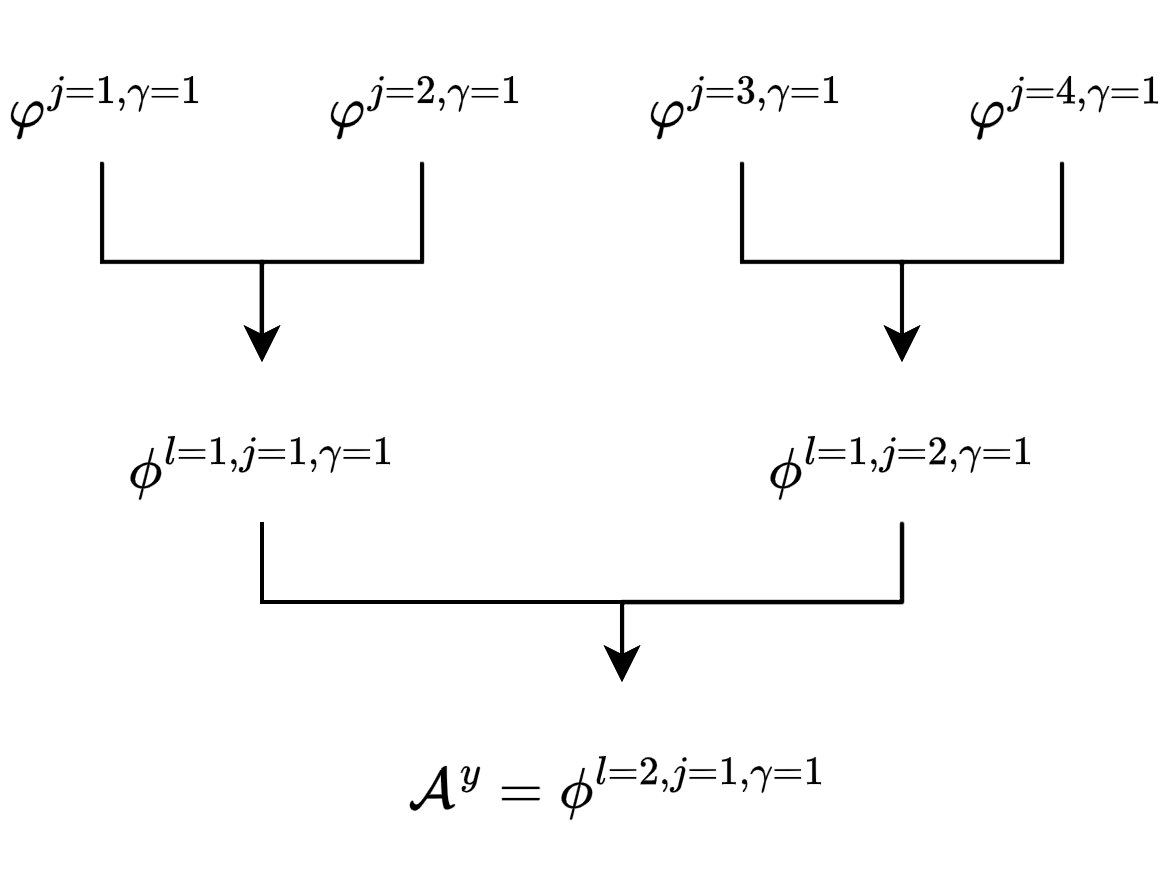
\includegraphics[width=0.6\textwidth]{matematicas/descomp_ht_rank_1}
    \caption{Ejemplo gráfico del proceso de construcción del tensor $\mathcal{A}^y$ a través de la descomposición \textit{HT}. Por simplicidad, estamos suponiendo que $r = 1$. Tenemos $L = 2$ capas o niveles}
    \label{img:diagrama_ht_simple}
\end{figure}

Veamos ahora este mismo diagrama, pero suponiendo que $r = 2$. Por tanto, en cada posición de cada nivel, tendremos dos tensores en vez de uno.

\begin{figure}[H]
\centering
    \ajustarsubcaptions
    \begin{subfigure}{.5\textwidth}
        \centering
        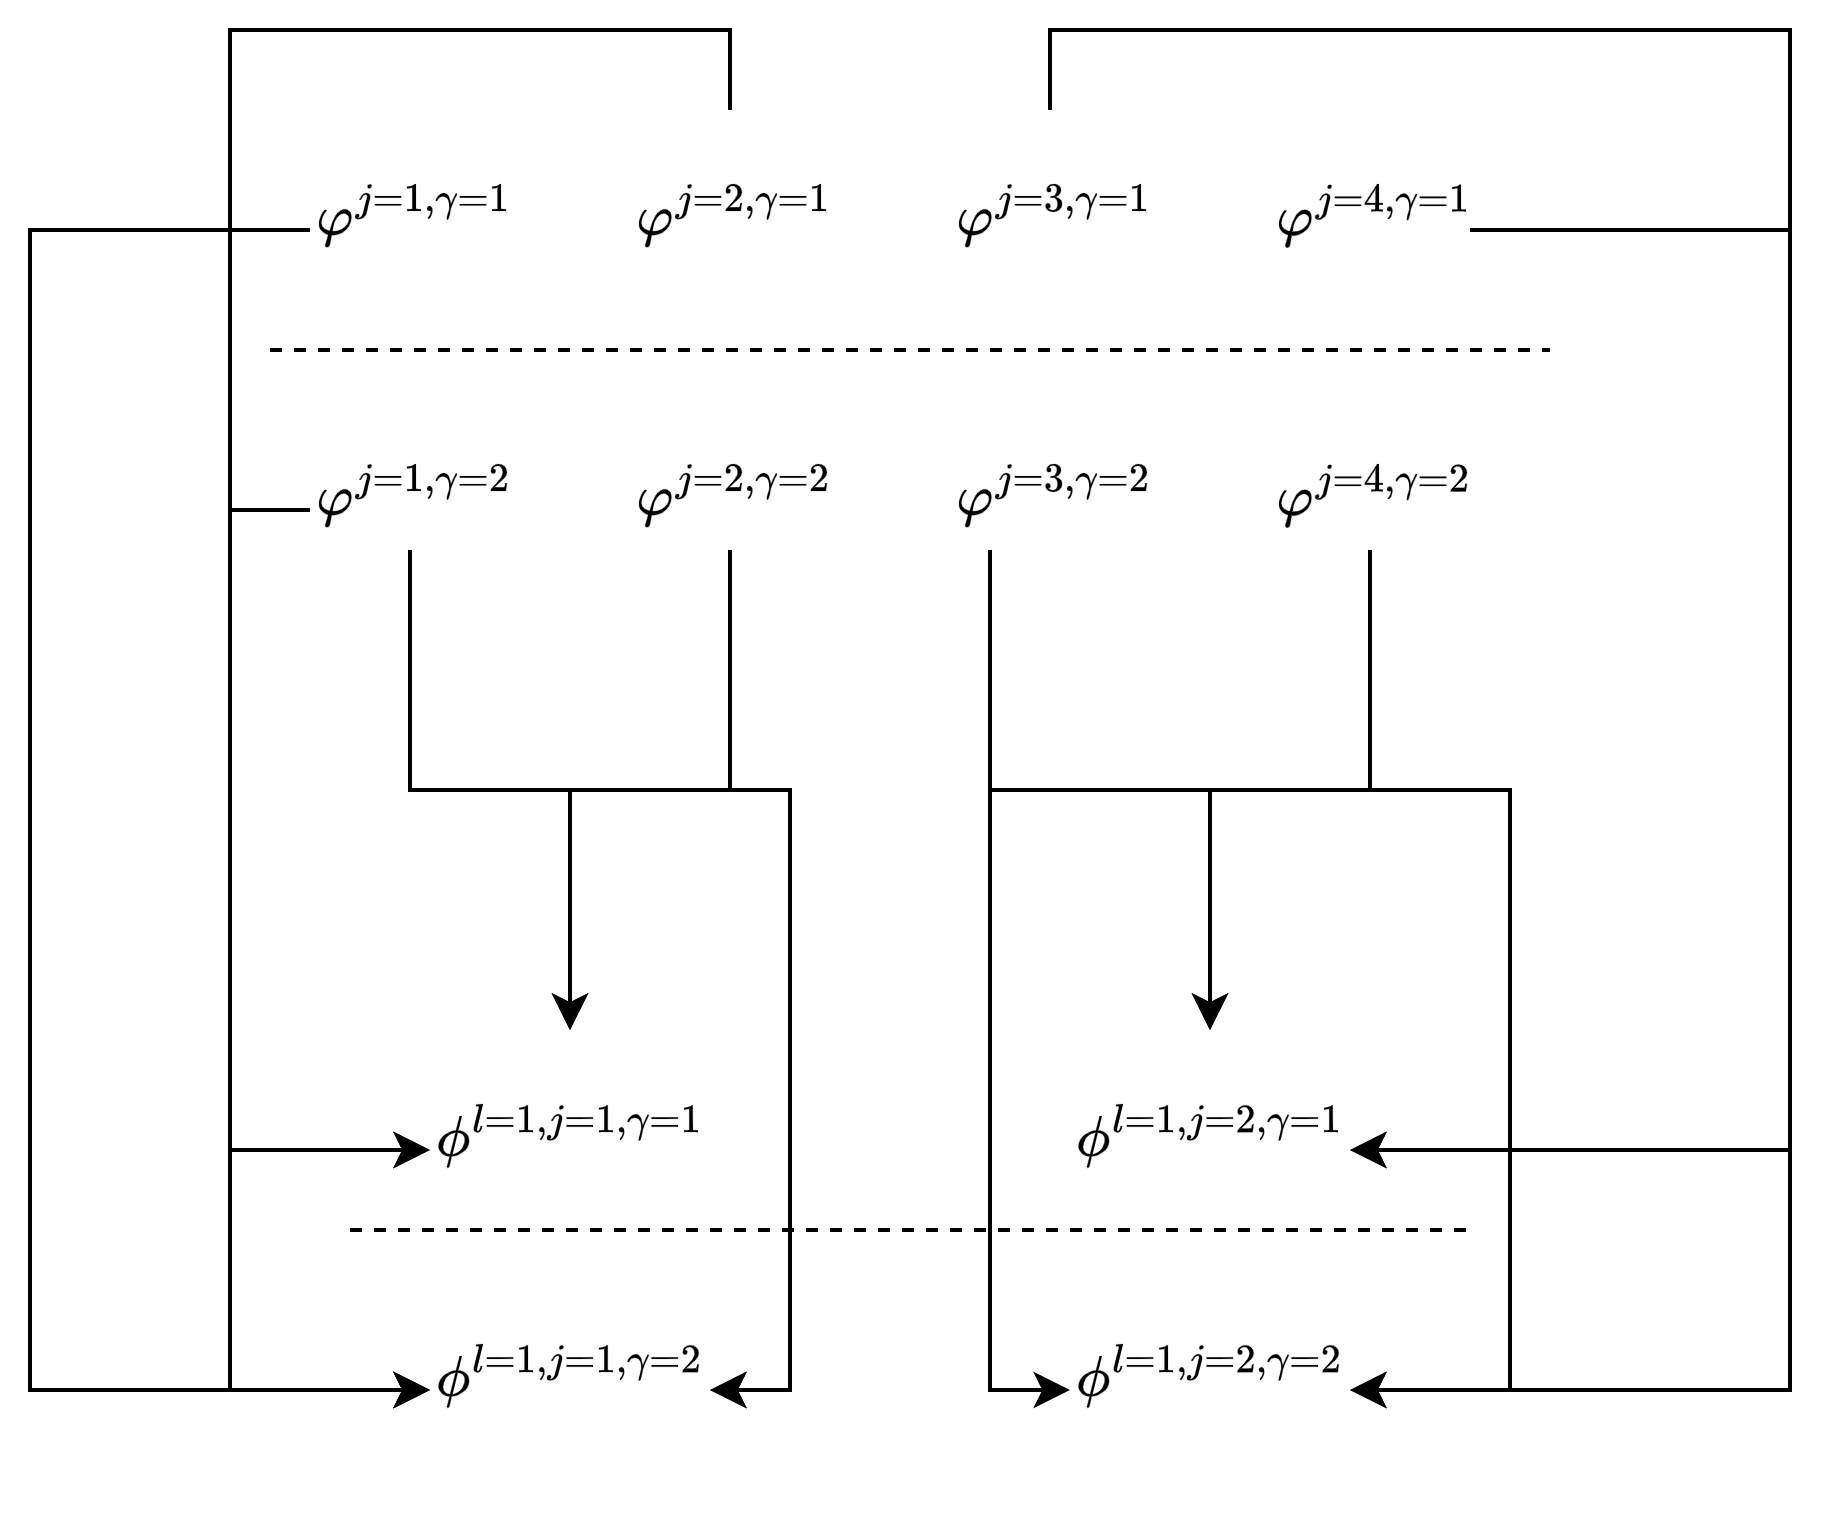
\includegraphics[width=0.9\linewidth]{matematicas/descomp_ht_rank_2_paso_1}
        \caption{Primer paso. En la construcción de cada tensor $\phi^{l, j, \gamma}$ participan cuatro tensores $\varphi^{j, \gamma}$}
    \end{subfigure}%
    \begin{subfigure}{.5\textwidth}
        \centering
        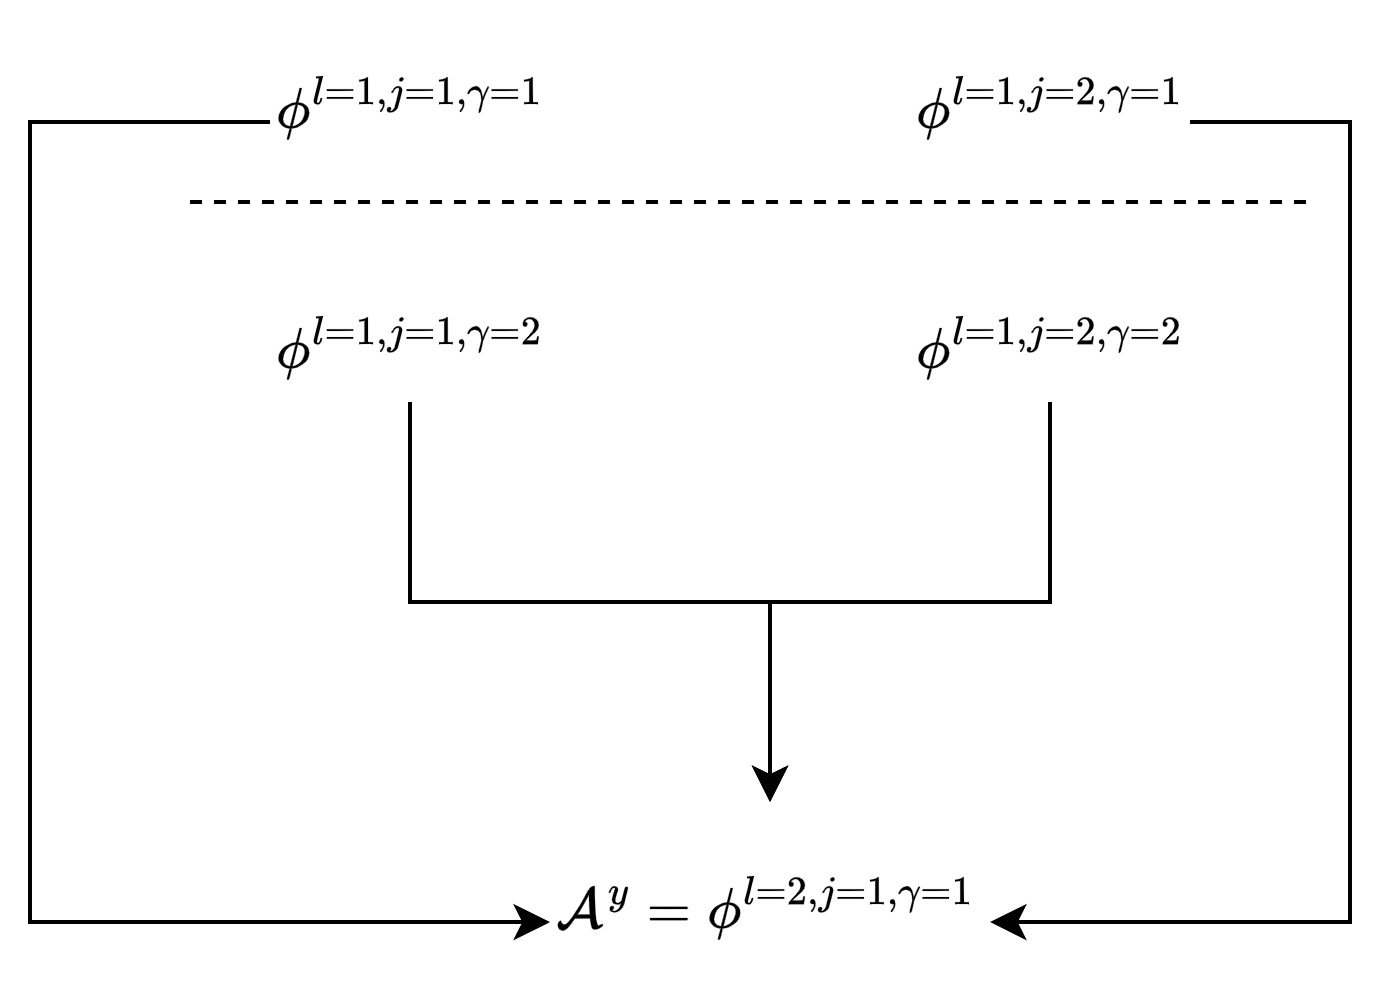
\includegraphics[width=0.9\linewidth]{matematicas/descomp_ht_rank_2_paso_2}
        \caption{Segundo paso. En la construcción del tensor $\mathcal{A}^y$ participan los cuatro tensores $\phi^{l=2, j, \gamma}$}
    \end{subfigure}
    \caption{Ejemplo gráfico del proceso de construcción del tensor $\mathcal{A}^y$ a través de la descomposición \textit{HT}. Hemos dividido el proceso de construcción en dos pasos. Ahora $r = 2$. Por lo tanto, en cada posición de cada capa, tenemos dos tensores. Seguimos teniendo $L = 2$ capas. }
    \label{img:diagrama_ht_complejo}
\end{figure}

\todo{Comentar en algún lado que $L = log_2(N)$. Además, estamos viendo en estos diagramas y en la ecuación principal \eqref{eq:descomposicion_ht} que estamos combinando dos a dos tensores, reduciendo en 2. Por eso es conveniente suponer que el orden de $\mathcal{A}^y$ es una potencia de dos}

\subsection{Parámetros del modelo} \label{msubs:parametros_modelo_ht}

Nuestro modelo viene dado por los siguientes parámetros:

\begin{itemize}
    \item Vectores iniciales:
        \begin{equation}
            \{\nv{\varphi^{j, \alpha}} \in \R^M: j \in \deltaset{N}, \alpha \in \deltaset{r_0}  \}
        \end{equation}

        Es decir, que aportan $M \cdot r_0 \cdot N$ coeficientes
    \item Pesos intermedios:

        \begin{equation}
            \{ a^{l, j, \gamma}_{\alpha} \in \R: l \in \deltaset{L-1}, j \in \deltaset{\frac{N}{2^l}}, \gamma \in \deltaset{r_l}, \alpha \in \deltaset{r_{l-1}} \}
        \end{equation}

        Por tanto, están aportando $\sum_{l = 1}^{L-1} r_{l-1} \cdot \frac{N}{2^l} \cdot r_l$ coeficientes.

    \item Pesos finales:

        \begin{equation}
            \{a^{L, y}_{\alpha}: y \in \deltaset{Y}, \alpha \in \deltaset{r_{L-1}} \}
        \end{equation}

        Por tanto, están aportando $r_{L-1} \cdot Y$ coeficientes.
\end{itemize}

Es decir, que nuestro modelo tiene

\begin{equation}
    M \cdot r_0 \cdot N + \sum_{l = 1}^{L-1} (r_{l-1} \cdot \frac{N}{2^l} \cdot r_l ) +
    r_{L-1} \cdot Y
\end{equation}

coeficientes. Si asumimos que todos los rangos son iguales, $r := r_0 = \ldots = r_{L-1}$, entonces el número de parámetros es:

\begin{equation}
\begin{split}
    M \cdot r \cdot N + \sum_{l = 1}^{L-1} r^2 \cdot \frac{N}{2^l} + r \cdot Y &= M \cdot r \cdot N + N \cdot r^2 \cdot \frac{2^{L-1} - 1}{2^{L-1}} + r \cdot Y \longmapsto \ldots \\
    \ldots & \encima{\longmapsto}{L \mapsto \infty} M \cdot r \cdot N + N \cdot r^2 + r \cdot Y
\end{split}
\end{equation}

donde hemos usado que:

\begin{equation}
    \sum_{l = 1}^{L-1} \frac{1}{2^l} = \frac{2^{L-1} - 1}{2^{L-1}}
\end{equation}

Podemos comprobar esto fácilmente:

\begin{proposicion}
    \begin{equation}
        \sum_{k = 1}^{N} \frac{1}{2^k} = \frac{2^N - 1}{2^N}; \dspace \forall N \in \N
    \end{equation}
\end{proposicion}

\begin{proof}
    Procederemos por inducción. Veamos que la ecuación se verifica para $N = 1$:

    \begin{equation}
        \sum_{k = 1}^{1} \frac{1}{2^k} = \frac{1}{2} = \frac{2^1 - 1}{2^1}
    \end{equation}

    Supuesto que la ecuación se cumple para $N$, veamos si la ecuación se cumple para $N + 1$:

    \begin{equation}
    \begin{split}
        \sum_{k = 1}^{N+1} \frac{1}{2^k} &= \sum_{k = 1}^{N} (\frac{1}{2^k}) + \frac{1}{2^{N+1}} \encima{=}{\text{hip. ind.}} \ldots \\
        \ldots &= \frac{2^N - 1}{2^N} + \frac{1}{2^{N+1}} = \ldots \\
        \ldots &= \frac{2^{N+1} - 2 + 1}{2^{N+1}} = \ldots \\
        \ldots &= \frac{2^{N+1} - 1}{2^{N+1}}
    \end{split}
    \end{equation}
\end{proof}
\todo{Tengo hecha esta demostración de forma directa en la página 49 de mis notas}

\todo{En el \textit{paper} esta ecuación la hacen igual a uno. Estoy bastante seguro de las cuentas pero no sé si me estoy confundiendo en algún detalle previo a plantear este paso}

\begin{proposicion}

    La descomposición \textit{HT} es universal. Es más, extiende la descomposición \textit{CP}. Esto es, cualquier tensor que pueda expresarse como la descomposición \textit{CP} con rango \textit{CP} $Z$, admite una descomposición \textit{HT} con rangos $r_1 = r_2 = \ldots = r_{L - 1} = Z$
\end{proposicion}

\begin{proof}

    \todo{En la página 8 del paper se da una indicación de cómo se hace esto}

\end{proof}

\begin{observacion}

    Aunque \textit{HT} sea una extensión de \textit{CP}, hay que tener en cuenta que el número de coeficientes crece.

    En el modelo \textit{CP} tenemos $N \cdot M \cdot Z + Z \cdot Y$ coeficientes que especificar (\customref{msubsec:parametros_modelo_cp}).

    En el modelo \textit{HT} tenemos $N \cdot M \cdot Z + N \cdot Z^2 \cdot \frac{2^{L-1} - 1}{2^{L-1}} + Z \cdot Y$, teniendo en cuenta que estamos considerando $r = Z$ (\customref{msubs:parametros_modelo_ht}).

    Por lo tanto, la diferencia en número de coeficientes viene dada por:

    \begin{equation}
        Z^2 \cdot \frac{2^{L-1} - 1}{2^{L-1}} \encima{\longmapsto}{L \mapsto \infty} N \cdot Z^2
    \end{equation}

    Por lo tanto, el número de parámetros crece de forma cuadrática. Sin embargo, como veremos más adelante, la ganancia en expresividad del modelo es exponencial.
    \todo{Revisitar esto cuando haya especificado formalmente qué significa ganancia exponencial en expresividad}

\end{observacion}

\subsection{Desarrollo del modelo}

El modelo \textit{HT} es el resultado de usar la descomposición \textit{HT} descrita en la ecuación \eqref{eq:descomposicion_ht} en nuestra función de puntuación \eqref{eq:puntuacion_general}. En esta sección, describiremos el modelo producido.

Como en el modelo \textit{CP}, el primer paso consiste en computar la capa de representación, $\{f_d(\nv{x_i}): d \in \deltaset{N}, i \in \deltaset{M}\}$. Tras la capa de representación, aplicamos las $L$ capas ocultas \eqref{eq:descomposicion_ht} que producen la salida.

Cada capa oculta se compone de una convolución $1 \times 1$ y un \textit{product pooling} con tamaño de ventana 2. En el modelo \textit{CP}, el \textit{product pooling} era global, colapsando las \textit{feature maps}. En este \textit{product pooling} reducimos el número de \textit{feature maps} a la mitad en cada paso.

Por lo tanto, tras las $L = log_2(N)$ capas ocultas, las $N$ \textit{feature maps} iniciales acaban siendo una sola. Por lo tanto, acabamos con una lista de $r_{L - 1}$ coeficientes sobre los que aplicamos una última capa oculta, dada por la última ecuación de \eqref{eq:descomposicion_ht}.

Nuestra red realiza \textit{product pooling} con un tamaño de ventana 2, sin \textit{overlapping} gracias al hecho de que estamos combinando los tensores dos a dos, de forma contigua, como indican \customref{img:diagrama_ht_simple} y \customref{img:diagrama_ht_complejo}. Como muestra \cite{matematicas:descomposicion_ht}, podríamos haber escogido otra forma de combinar los tensores. Por ejemplo, combinando más de dos en cada paso. Esto produciría diferentes combinaciones de tamaños de ventana en el \textit{product pooling} y, por tanto, distintas profundidades.


\todo{Escribir esta capa de representación}

\todo{Escribir en algún lugar que $L = log_2(N)$}

\todo{Es muy mal nombre}

\todo{Revisar la escritura de este apartado, porque es muy importante en el \textit{TFG}}




\setpartpreamble[c][0.75\linewidth]{
    % Deja un espacio vertical en la parte superior
	\bigskip

    En esta segunda parte del trabajo, introduciremos un nuevo método para computar el \entrecomillado{Triplet Loss}. Aplicaremos este nuevo método a una tarea de reconocimiento facial invariante a cambios de edad, y justificaremos por qué esta técnica parece no ser adecuada para resolver este problema
    % \todo{Revisar esta brevísima introducción porque la escribo al principio. Igual cuando lleve más escrito este enfoque ha cambiado}
}
\cleardoublepage\part{Segunda parte}

\chapter{Introducción}\label{ch:introduccion}

El objetivo de este trabajo, desde la perspectiva de las matemáticas, es \textbf{analizar las redes neuronales profundas basadas en convoluciones y explicar por qué en ciertos escenarios éstas funcionan mejor que las redes neuronales no profundas}, a las que llamaremos redes someras. En este escenario ocurre que para replicar redes profundas con un número polinomial de coeficientes, necesitamos que las redes someras tengan un número de coeficientes superior al polinomial, concretamente, exponencial. En este caso hablamos de \textbf{eficiencia en profundidad} o \textbf{\entrecomillado{depth efficiency}}.
\todo{Poner aquí una referencia a otra parte del paper sobre esto de tamaño exponencial}

La eficiencia en profundidad es muy conocida en la práctica, pero pocos son los trabajos que han tratado de justificar matemáticamente por qué ocurre este fenómeno. Además, como se comenta en \cite{matematicas:principal}, \textbf{en la mayoría de trabajos de este tipo, no se han tenido en cuenta propiedades fundamentales de las redes profundas ni de las redes convolucionales} \cite{matematicas:paper_depth_malo_01} \cite{matematicas:paper_depth_malo_02} \cite{matematicas:paper_depth_malo_03}. Por otro lado, suelen ser trabajos en los que \textbf{se muestran ejemplos concretos} de funciones implementables (de forma eficiente) con redes profundas pero no con redes someras, sin dar \textbf{ningún tipo de información sobre con qué frecuencia ocurre esto}. En base a esto, las \textbf{principales fortalezas de este trabajo respecto a otros} es que consideramos:
\todo{Comentarios de JMeri: este tipo de afirmaciones pueden llevar a preguntas del tribunal. Preparar bien las posibles respuestas}
\todo{Quizás yo añadir comentarios sobre esta afirmación para que se responda automáticamente al leer esto}

\begin{itemize}
	\item La diferencia jerárquica entre ambos tipos de redes.
	\item Propiedades fundamentales de las redes convolucionales: compartición de los coeficientes en las convoluciones, localidad de la operación de convolución y uso de la operación de \textit{pooling}.
	\item Un estudio de lo frecuente que es tener funciones que sean implementables (de forma eficiente) por redes profundas pero no por redes someras.
\end{itemize}
\todo{Desarrollar más qué significan estas propiedades. En la introducción del paper se explica esto más o menos}

\section{Objetivos}

Los principales \textbf{objetivos} del presente trabajo son los siguientes. Como punto de partida, modelar matemáticamente la tarea de aprendizaje representando los datos de entrada, la tarea a resolver y el espacio de hipótesis en el que buscaremos la mejor solución. Posteriormente, modelar los dos tipos de redes neuronales (profundas y someras) a través de dos tipos de descomposiciones tensoriales. La descomposición \textit{CP}, que equivale al uso de redes someras y que desarrollamos en la \sectionref{subs:descomposcion_cp}. Y la descomposición \textit{HT}, que equivale al uso de redes profundas y que introducimos en la \sectionref{subs:descomposicion_ht}. Finalmente, demostrar dos resultados centrales que pondrán de manifiesto la superioridad de las redes profundas, en lo que se conoce como eficiencia en profundidad, a través de las ya mencionadas descomposiciones tensoriales.

El primer resultado central, el \propref{teorema:teorema_principal_especificacion}, dice que si tenemos un modelo profundo con un número polinomial de coeficientes, el modelo somero necesitará al menos un número exponencial de coeficientes para poder implementar el mismo modelo. Esto ocurre casi por doquier respecto al espacio de los coeficientes que determinan el modelo profundo. El segundo resultado central, el \propref{corolario:corolario_principal_concreto}, indica que no es que un modelo somero no pueda realizar el modelo profundo con menos de un número exponencial de parámetros, sino que no es capaz ni de aproximar al modelo profundo con menos de un número exponencial de parámetros. De nuevo, esto ocurre casi por doquier respecto al espacio de los coeficientes que determinan el modelo profundo.

Nos basaremos principalmente en el trabajo \cite{matematicas:principal}. Algunas de las herramientas que usaremos serán la teoría básica sobre tensores, las descomposiciones tensoriales \textit{CP} y \textit{HT}, la matrización de tensores, algunos resultados conocidos sobre la medida de Lebesgue y finalmente el álgebra de matrices básica.

\section{Estructura del trabajo}

La estructura del trabajo será la siguiente. En primer lugar, en el \sectionref{ch:matematicas_fundamentales} introduciremos las herramientas básicas sobre las que fundamentaremos nuestro trabajo. En concreto, introduciremos el concepto de producto tensorial. En segundo lugar, en el \sectionref{ch:tarea_aprendizaje} indicaremos cómo representamos matemáticamente la tarea de aprendizaje. Para ello, modelizaremos un espacio de hipótesis general, para lo cual justificaremos la elección de ciertas funciones de puntuación, que serán clave en el desarrollo del trabajo, y la elección de determinadas funciones de representación. En la \sectionref{subs:capa_de_representacion} daremos un primer paso común en la modelización de ambas arquitecturas de aprendizaje automático, presentando la primera capa de ambos modelos. En tercer lugar, en el \sectionref{ch:modelizacion} desarrollaremos las dos modelizaciones (somera y profunda) a partir de dos descomposiciones tensoriales (\textit{CP} y \textit{HT}, respectivamente). Veremos en ambos casos cómo las modelizaciones realizadas se corresponden con arquitecturas usadas en la práctica del aprendizaje automático. Compararemos el número de parámetros que definen cada modelo, pues será fundamental en nuestros resultados teóricos. En cuarto lugar, en el \sectionref{chapter:teoremas_y_demostraciones} introduciremos los dos resultados principales, veremos y demostraremos algunos resultados previos necesarios para las demostraciones y probaremos el teorema y corolario principal. En quinto y último lugar, en el \sectionref{chapter:conclusiones_trabajo_futuro} comentaremos los resultados obtenidos a partir del presente trabajo e introduciremos posibles líneas de estudio en base a nuestros resultados.

\chapter{Fundamentos teóricos} \label{ich:fundamentos_teoricos}

En esta sección introduciremos algunos \textbf{conceptos teóricos} sobre los que se basará nuestro trabajo, y por tanto, conviene conocer para entender este trabajo.

\section{\textit{Embeddings}} \label{isec:embeddings}

Nuestro trabajo busca desarrollar un modelo de aprendizaje automático que aprenda un \textit{embedding}. Un \textit{embedding} no es más que un mapeo desde un cierto espacio $X$ de datos de entrada (en nuestro caso, podemos considerar $X$ como el espacio de imágenes en las que aparecen caras) a un espacio vectorial $\R^N$. En la mayoría de casos, la dimensión del espacio de llegada $N$ es menor que la dimensión del espacio $X$.

Más formalmente, buscamos aprender una función

\begin{equation}
\begin{split}
    f_{\theta}: X & \to \R^N \\
    x & \mapsto f_{\theta}(x)
\end{split}
\end{equation}

que tomamos de una familia paramétrica de funciones $\{f_{\theta}: \theta \in \Theta \}$. En el caso de nuestro problema, podemos pensar en la familia de los modelos profundos de redes convolucionales ($\theta$ estaría por tanto compuesto por todos los coeficientes que determinan dicho modelo convolucional, luego podríamos pensar en $\Theta \subseteq \R^M$ donde $M$ es el número de coeficientes del modelo).

El criterio para escoger una función u otra de mapeo es que este deberá ser \textbf{semántico}. En el espacio de llegada $\R^N$ tenemos una métrica:

\begin{equation}
\begin{split}
    D: X \times X & \to [0, \infty) \\
    x, y & \mapsto D(x, y)
\end{split}
\end{equation}

Por ejemplo, la métrica euclídea. Queremos que \textbf{datos semánticamente relacionados en $X$ sean mapeados a vectores en $\R^N$ cercanos} por la métrica que fijemos. Del mismo modo, datos semánticamente distintos deberán ser mapeados a vectores distantes.

Además, será deseable que $f_{\theta}$ sea una función continua (en casi cualquier ámbito podemos considerar $X = \R^M$ para algún valor de $M$). Por ejemplo, en el caso de las imágenes, un ligero cambio en un \textit{píxel} de la imagen no debería producir un vector muy distanciado del original. En muchas ocasiones, al estar buscando que el \textit{embedding} sea semántico, esta restricción inducirá en menor o mayor medida dicha continuidad.

\begin{ejemplo}
    Consideremos que queremos computar un \textit{embedding} para representar palabras.

    Este problema es \textbf{especialmente relevante} en el ámbito del lenguaje natural. Esto es así porque, si queremos trabajar con texto usando modelos de aprendizaje automático, deberemos primero convertir dicho texto a una representación numérica. Usar, por ejemplo, el código binario que codifica dicho texto no parece muy buena idea, porque este mapeo no es semántico ni continuo.

    En este caso, queremos que palabras con una semántica parecida se transformen a vectores cercanos. Por ejemplo, la distancia entre los \textit{embeddings} de las palabras \entrecomillado{ciudad}, \entrecomillado{pueblo} debería ser mucho menor que la distancia entre los \textit{embeddings} de las palabras \entrecomillado{papel}, \entrecomillado{odio}. Esta idea se puede visualizar en la siguiente representación:

    \begin{figure}[H]
        \centering
        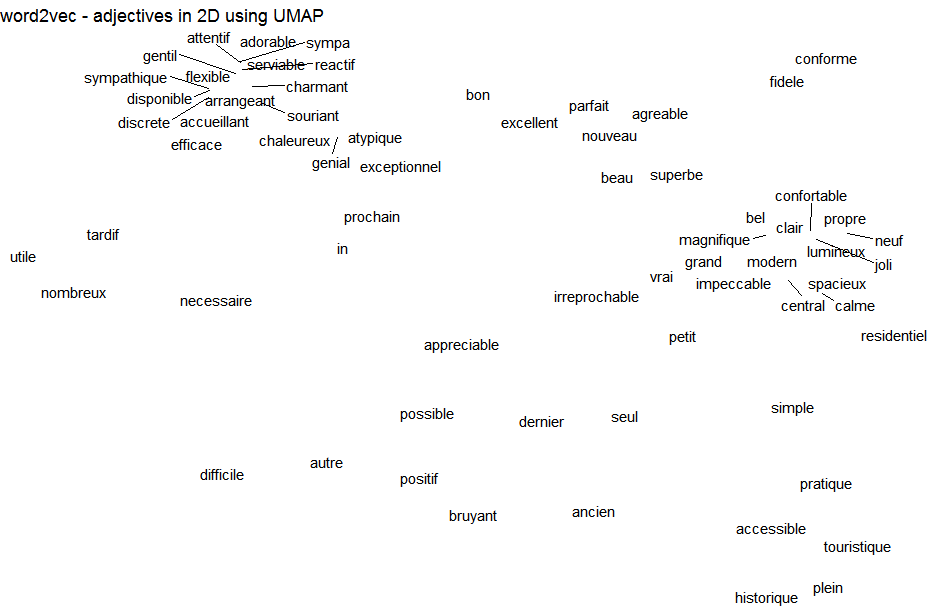
\includegraphics[width=0.6\textwidth]{informatica/word2vec_example}
        \caption{Ejemplo de un \textit{embedding} semántico, computado por el modelo \textit{word2vec} \cite{informatica:word2vec}, de palabras en francés. Imagen extraída de \url{https://cran.r-project.org/web/packages/word2vec/readme/README.html}}
    \end{figure}

    En el caso concreto de \cite{informatica:word2vec}, que propone el conocido modelo \textit{word2vec}, se consigue que el \textit{embedding} tenga cierta \entrecomillado{estructura algebraica}, pudiendo computar, por ejemplo:

    \begin{equation}
        vector("rey") - vector("hombre") + vector("mujer") = vector("reiina")
    \end{equation}
\end{ejemplo}

\begin{ejemplo}
    Veamos ahora un ejemplo mucho más cercano con el problema que queremos resolver. Por ejemplo, el problema de re-identificación (ambiente en el que se proponen las nuevas técnicas de cómputo del \textit{triplet loss} \cite{informatica:principal}).

    En este caso, queremos que las imágenes de una persona en una escena, se transformen a vectores cercanos, como muestra la siguiente representación:

    \begin{figure}[H]
        \centering
        \includegraphics[width=0.6\textwidth]{informatica/embedding_paper_principal}
        \caption{Imagen extraída de \cite{informatica:principal}. Se representa una proporción del \textit{dataset} \textit{Market-1501} tras aplicar el \textit{embedding} aprendido y posteriormente \textit{t-SNE}}
    \end{figure}

    Por ejemplo, un modelo que quiera resolver esta tarea podría aprender a mapear personas con exactamente la misma ropa a puntos cercanos.
\end{ejemplo}

\begin{ejemplo}

    Y para finalizar, consideremos nuestra tarea en concreto. Buscamos que las imágenes de la misma persona, aunque hayan pasado los años, se transformen en vectores cercanos. Y al contrario, que imágenes de dos personas distintas estén lo más lejos posible.

    Esto es especialmente complicado, como ya hemos comentando en \customref{ich:descrp_problema}, porque por ejemplo, nuestro modelo debe ver como más cercanos imágenes de un niño y un adulto con barba (ambos siendo la misma persona) que dos imágenes de dos adultos con barba (siendo distintas personas), como hemos mostrado claramente en \customref{img:messi_distintos_otro_adulto}

\end{ejemplo}

\section{\textit{Triplet Loss}} \label{isec:triplet_loss}

Nuestro objetivo es ahora justificar el uso de \textit{triplet loss} como una función de pérdida que permita a nuestro modelo aprender un \textit{embedding} semántico.

Recordemos que estamos trabajando con funciones de la forma:

\begin{equation}
\begin{split}
    f_{\theta}: X & \to \R^N \\
    x & \mapsto f_{\theta}(x)
\end{split}
\end{equation}

y con una métrica:

\begin{equation}
\begin{split}
    D: X \times X & \to [0, \infty) \\
    x, y & \mapsto D(x, y)
\end{split}
\end{equation}

Para ser más concisos, usaremos la notación $D_{i, j} := D(f_{\theta}(x_i), f_{\theta}(x_j))$.

Como su nombre indica, \textit{triplet loss} trabajará sobre triples. Esto es:

\begin{enumerate}
    \item Una imagen de un individuo concreto, a la que llamaremos \textbf{\textit{anchor}} o ancla
    \item Otra imagen distinta, pero del mismo individuo, a la que llamaremos \textbf{positivo}
    \item Una imagen de un individuo distinto, a la que llamaremos \textbf{negativo}
\end{enumerate}

En este caso, queremos que la distancia entre el \textit{embedding} del ancla y el positivo (que podemos denotar $D_{A, P}$) sea mucho menor que la distancia entre el \textit{embedding} del ancla y el negativo (denotamos $D_{A, N}$). Por tanto, lo que realmente queremos es que:

\begin{equation}
    D_{A, P} \leq D_{A, N}
\end{equation}

o lo que es lo mismo,

\begin{equation}
    D_{A, P} - D_{A, N} \leq 0
\end{equation}

Una forma trivial de hacer que esa ecuación se cumpla, es haciendo que

\begin{equation}
    f(x) = \vec{0}; \dspace \forall x \in X
\end{equation}

con lo que obtendríamos un modelo totalmente inservible. Para evitar eso, introducimos un término $\alpha > 0$ que se conoce como \textbf{margen}, llegando a:

\begin{equation}
    D_{A, P} - D_{A, N} + \alpha \leq 0
\end{equation}

Buscamos que el término de la izquierda sea lo más negativo posible, por lo buscamos minimizar la siguiente función de pérdida:

\begin{equation} \label{ieq:triplet_loss_single_entry}
\begin{split}
    \mathcal{L}_{tri}(\theta; A, P, N) & := max \{D_{A, P} - D_{A, N} + \alpha, 0 \} = \ldots \\
    \ldots &= ReLU(D_{A, P} - D_{A, N} + \alpha)
\end{split}
\end{equation}

Minimizando esta función de pérdida, lo que haremos será atraer elementos de la misma clase entre sí, y alejar elementos de clases distintas. Este proceso se refleja en la siguiente imagen:

\begin{figure}[H]
    \centering
    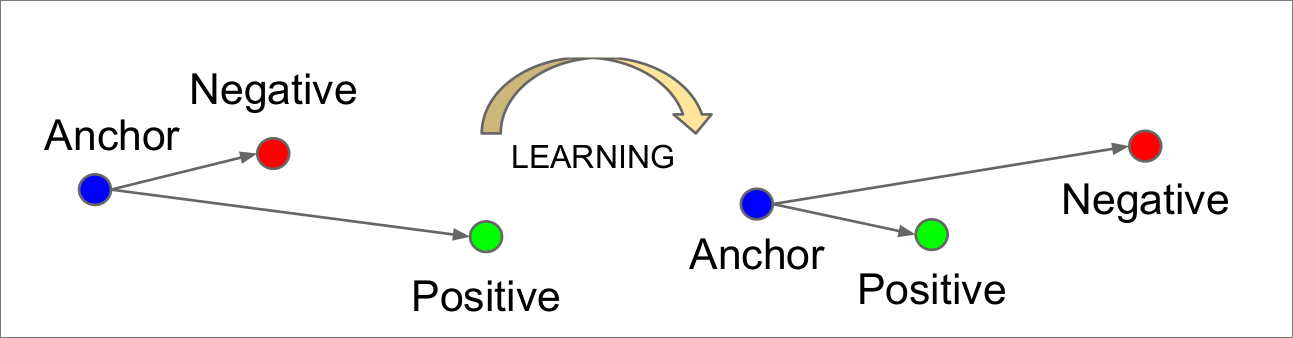
\includegraphics[width=0.8\textwidth]{informatica/triplet_loss_learning}
    \caption{Ejemplo gráfico del proceso de aprendizaje deseado con \textit{triplet loss}. Imagen extraída de \cite{informatica:facenet}}
\end{figure}

Sin embargo, en \eqref{ieq:triplet_loss_single_entry} trabajamos con una sola entrada de tres datos. A diferencia de un \textit{dataset} con datos etiquetados clásico (de la forma \lstinline{(entrada, valor de etiqueta)}), tenemos datos de la forma \lstinline{(imagen, identificador de individuo, edad)}. Esto supone un \textbf{problema} a resolver: cómo generamos \textit{batches} con triples de la forma \lstinline{(ancla, positivo, negativo)} para poder aplicar \eqref{ieq:triplet_loss_single_entry}. Introducimos algunas soluciones propuestas a este problema en \customref{isec:batching}

Por otro lado, este enfoque plantea algunas \textbf{ventajas}. La principal es que, a diferencia de otros enfoques basados en usar funciones de pérdida auxiliares (y que suelen fuerzan que la red solo pueda funcionar comparando pares de imágenes), el cómputo del \textit{embedding} es directo usando esta función de pérdida (\textit{end to end learning}). Optimizamos directamente la propiedad semántica del \textit{embedding} que deseamos obtener. Una vez entrenado el modelo es directo adaptar el modelo a tareas de \textit{clustering}, \textit{retrieval}, verificación, \ldots \cite{informatica:principal}

\section{Generación de \textit{batches}} \label{isec:batching}

Como ya hemos comentado, la tarea que debemos resolver ahora es la de generación de \textit{batches} adecuados para poder emplear \eqref{ieq:triplet_loss_single_entry} como función de pérdida a minimizar.

Por tanto, dado un conjunto de datos de la forma \lstinline{(imagen, identificador, edad)}, debemos obtener un conjunto de datos de la forma \lstinline{(img. ancla, img. positivo, img. negativo)}. Este último conjunto de datos puede ser una lista de triples o conjuntos de \textit{batches}. Como vamos a trabajar con \textit{batches}, podemos simplemente muestrear aleatoriamente y sin remplazo de la lista de triples, repitiendo el muestreo tras cada época completada.

\subsection{Enfoque \textit{offline}} \label{isubs:enfoque_offline_minado_triples}

Este es el enfoque clásico, que se ha venido usando previo a \cite{informatica:facenet}, que introduce un enfoque \textit{online} que luego otros trabajos como \cite{informatica:principal} han ido mejorando.

En este enfoque, el ciclo de aprendizaje se divide en \textbf{varios pasos}.

En primer lugar, se realiza un \textbf{minado \textit{offline}} de los triples. Es decir, se obtiene una primera lista (o conjunto de \textit{batches}) de la forma \lstinline{(img. ancla, img.positivo, img.negativo)}. Una forma de hacer esto sería, por ejemplo, generar los triples de forma aleatoria, generar todos los posibles triples, $\ldots\dspace$ Aunque estas ideas no suelen funcionar en la práctica. Otra forma más efectiva es seleccionar los triples en base de algún estudio estadístico. O usar la red que vamos a optimizar, para identificar aquellos triples en los que tiene más dificultad de distinguir.

En segundo lugar, realizamos el aprendizaje sobre dicho conjunto de triples. En algunos casos, realizamos el entrenamiento completo sobre dicho conjunto inicial. En otros casos, principalmente cuando usamos la red para el minado de triples, pasadas algunas épocas de entrenamiento volvemos a generar otra vez la lista de triples. Así, triples que antes la red no identificaba propiamente, ahora sí que los identifica (\entrecomillado{network snapshots}, \cite{informatica:facenet}) y podemos buscar triples más interesantes.

Una vez computado una lista de triples $(a, p, n) \in \Omega$, la función de pérdida \eqref{ieq:triplet_loss_single_entry} se implementa de forma natural como en cualquier otro ámbito de \textit{batching}:

\begin{equation}
    \mathcal{L}_{tri}^{offline}(\theta; \Omega) := \frac{1}{\#\Omega} \sum_{(a, p, n) \in \Omega} \mathcal{L}_{tri}(\theta; a, p, n)
\end{equation}

\begin{observacion}

Normalmente, en la literatura sobre aprendizaje automático, se ignora el término $\frac{1}{\#\Omega}$ y se supone que siempre estamos dividiendo por el número de sumandos, con lo que nuestra función de error suele escribirse como:

\begin{equation}
    \mathcal{L}_{tri}^{offline}(\theta; \Omega) := \sum_{(a, p, n) \in \Omega} \mathcal{L}_{tri}(\theta; a, p, n)
\end{equation}


\end{observacion}

Este enfoque supone una serie de \textbf{problemas}:

\begin{itemize}
    \item Estamos dividiendo el proceso de aprendizaje en dos etapas, la de minado de triples y la de aprendizaje sobre estos triples. Esto añade complejidad a nuestra \textit{pipeline}
    \item La adecuada elección de triples es fundamental. Si elegimos triples demasiado fáciles, la red no aprenderá nada nuevo, pues es muy fácil distinguir los ejemplos presentados. Sin embargo, si solo mostramos triples complicados, el modelo se centrará en aprender ejemplos extraordinarios y no sabrá distinguir el grueso de ejemplos más sencillos
        \begin{itemize}
            \item Además, generalmente los modelos aprenden rápidamente a distinguir la mayoría de ejemplos en los que las diferencias son relativamente evidentes. Por tanto, en pocas iteraciones la mayoría de triples son demasiado sencillos, lo que agrava mucho este problema
        \end{itemize}
    \item Lo ideal sería disponer de alguna forma de ajustar la complejidad de los triples presentados. Podemos confiar en que al ir re-generando la lista de triples, la complejidad vaya aumentando. Pero el algoritmo de minado debería tener alguna forma de controlar el énfasis que se hace en la búsqueda de combinaciones difíciles, lo que añade aún más complejidad al sistema
    \item El minado supone realizar un proceso de búsqueda, que es \textbf{muy lento} (evaluar de alguna forma todos los posibles triples supondría al menos $O(n^3)$). Lo ideal sería disponer de algún método que se basará en muestrear aleatoriamente de nuestra lista de \lstinline{(imagen, identidad, edad)} (proceso que es muy rápido) y generar rápidamente triples interesantes (esto es lo que hacemos en \customref{isubs:triples_online})
\end{itemize}

\subsection{Enfoque \textit{online}} \label{isubs:triples_online}

La idea común será implementar el siguiente proceso. En primer lugar, realizaremos un muestreo aleatorio sobre los datos de la forma \lstinline{(imagen, identidad, edad)}. Este muestreo es rápido y no supone prácticamente tiempo de cómputo. Usando únicamente los datos de ese muestreo, generaremos triples y computaremos la función de pérdida apoyándonos en \eqref{ieq:triplet_loss_single_entry}. Dicha generación ya sí que supone un tiempo de cómputo considerable. Repetimos este proceso hasta agotar todos las entradas de nuestro \textit{dataset}, completando así una época de entrenamiento.

Ya podemos ver algunas \textbf{ventajas de este método}, incluso antes de haber especificado las dos partes fundamentales (muestreo y selección de triples):

\begin{enumerate}
    \item La ventaja más obvia es que, suponiendo que el tamaño de la muestra es significativamente mucho más pequeño que el tamaño de todo el conjunto de datos, la generación de triples consumirá potencialmente menos tiempo y será más efectiva
        \begin{itemize}
            \item Para afirmar esto rotundamente, tendríamos que realizar un estudio del tiempo del minado \textit{offline} en contraste a la suma de todos los tiempos de minado en cada muestreo
            \item Sin embargo, el tiempo usado es más eficiente, porque en cada paso estamos usando la red actualizada. En el minado \textit{offline} podemos gastar muchísimo tiempo en encontrar triples difíciles que, tras entrenar en pocos ejemplos previos, acaben siendo sencillos, y por tanto, cuando la red vea estos ejemplos, ya sean totalmente inútiles
        \end{itemize}
    \item Se facilita en gran parte el ajuste de la dificultad. Podemos buscar triples realmente difíciles, pero como solo se tiene acceso a una pequeña muestra, estamos controlando la dificultad. Aquí podemos variar el tamaño de las muestras para buscar un punto medio entre ejemplos muy difíciles o ejemplos demasiado sencillos. Y todo esto sin contar con el factor de que vamos a usar la red actualizada para la elección de los triples, como comentaremos más adelante
\end{enumerate}

Desarrollada esta visión de forma general, veamos cómo se implementa cada una de las partes, siguiendo las técnicas introducidas en \cite{informatica:principal}.

\subsection{Muestreo de los datos con \textit{P-K sampling}}

La \textbf{idea principal del muestreo} es lo que definiremos como \textbf{\textit{P-K sampling}}. Como ya hemos comentado en \customref{isubs:triples_online}, nuestra tarea ahora es generar un \textit{batch} de elementos de la forma \lstinline{(imagen, identidad, edad)}. En una segunda etapa (véase \customref{isubs:seleccion_de_triples}), otro algoritmo decide como generar triples a partir de estos datos.

El algoritmo de muestreo \textit{P-K sampling} es muy sencillo. En cada muestreo, seleccionamos aleatoriamente $P$ identidades de individuos (o clases, en un ambiente más general en el que no necesariamente estemos trabajando con imágenes de personas). Por cada una de las identidades, seleccionamos aleatoriamente $K$ imágenes. Por tanto, obtenemos una lista de $P \cdot K$ imágenes, o lo que podemos llamar, un \textbf{\textit{P-K batch}}. Para poder obtener triples interesantes en la siguiente etapa, parece que lo deseable es que ambas selecciones aleatorias (muestreos) sean sin repetición.

El hecho de tener $K$ imágenes por cada uno de los individuos seleccionados es lo que va a permitir al algoritmo de generación de triples obtener rápidamente triples interesantes.

Queda aquí claro los problemas que introduce este muestreo: si queremos muestrear $K$ imágenes de cada individuo sin repetición, cada individuo debe tener asociadas al menos $K$ imágenes. Así que a la hora de trabajar con un \textit{dataset}, siempre deberíamos comprobar la distribución del número de imágenes por individuo, como hemos hecho en \customref{isec:base_datos_usada}.

\subsection{Selección de triples y funciones de pérdida} \label{isubs:seleccion_de_triples}

Una vez que tenemos un \textit{batch} de $P \cdot K$ elementos, deberemos seleccionar triples de ellos. Una vez se especifica cómo se seleccionan los triples, usando \eqref{ieq:triplet_loss_single_entry}, inducimos de forma natural y directa una cierta función de pérdida que actúa sobre estos \textit{P-K batches}.

\begin{observacion}

    Vamos a trabajar con $P \cdot K$ elementos, cada uno correspondiendo a una clase en concreto. Por tanto, indexaremos los elementos de la forma $x_k^p$ donde $p$ marca el identificador del individuo, y $k$ marca a cuál de las $K$ imágenes del individuo $p$ nos estamos refiriendo

\end{observacion}

\subsubsection{\textit{Batch Hard}} \label{isubsubs:batch_hard}

La primera idea es iterar sobre todos los elementos del \textit{P-K batch}, obteniendo así $P \cdot K$ anclas. Por cada ancla, seleccionamos el positivo y negativo \textbf{más complicado dentro de \textit{P-K batch}}. Por tanto, queda claro que \textbf{estamos usando la red para seleccionar triples difíciles} en cada \textit{batch} generado.

Esto introduce la siguiente función de pérdida, a la que llamaremos \textbf{\textit{Batch Hard}}:

\begin{equation}
    \mathcal{L}_{BH}(\theta, \hat{\Omega}) := \comentarencima{\sum_{p = 1}^P \sum_{k = 1}^K}{\text{todas las anclas}} [
        \comentarencima{\max_{k' = 1, \ldots, K} D(f_{\theta}(x_k^p), f_{\theta}(x_{k'}^p))}{\text{positivo más complicado}}
        - \comentarencima{\min_{\substack{p' = 1, \ldots, P \\ p' \neq p \\ k' = 1, \ldots, K}} D(f_{\theta}(x_k^p), f_{\theta}(x_{k'}^{p'}))}{\text{negativo más complicado}}
        + \alpha]_+
\end{equation}

donde $[x]_+ := max \{0, x\} = ReLU(x)$ y $\hat{\Omega}$ se refiere a un \textit{P-K batch}. No olvidemos que no estamos escribiendo la división por el número de sumandos, $P \cdot K$.

Estamos generando \textbf{triples moderados}, porque estamos buscando los triples más difíciles, pero dentro de un \textit{batch} relativamente pequeño comparado a el total del conjunto de datos. Por tanto, estamos ajustando la dificultad de los triples cómodamente, resolviendo el problema que comentábamos en \customref{isubs:enfoque_offline_minado_triples}. Aumentando el valor de $P, K$, aumentamos el espacio de búsqueda, y por tanto podremos encontrar triples mucho más difíciles. Sin embargo, hay que tener siempre en cuenta el coste en tiempo de cómputo.

Queda claro que, gracias al proceso de \textit{P-K sampling}, ahora es factible realizar una búsqueda de triples interesantes en profundidad, basándonos en el estado más actualizado de la red para calcular la dificultad de los triples. Esta búsqueda extensiva no habría sido posible si la planteásemos sobre todo el conjunto de datos.

\subsubsection{\textit{Batch All}} \label{isubsubs:batch_all}

Motivados por lo comentado en \customref{isubsubs:batch_hard}, podemos plantearnos usar todas los posibles triples dentro de un \textit{P-K batch} como un enfoque que ahora cobra más sentido (ya hemos comentado en \customref{isubs:enfoque_offline_minado_triples} que realizar esto sobre todo el conjunto de datos no parece una buena idea).

Realizar esto introduce la función de pérdida que llamaremos \textbf{\textit{Batch All}}:

\begin{equation} \label{ieq:batch_all}
    \mathcal{L}_{BA}(\theta; \hat{\Omega}) :=
    \comentarencima{\sum_{p = 1}^{P} \sum_{k = 1}^K}{\text{todas anclas}}
    \comentardebajo{\sum_{\substack{k' = 1 \\ k' \neq k}}^{K}}{\text{todas pos.}}
    \comentarencima{\sum_{\substack{p' = 1 \\ p' \neq p}}^P \sum_{n = 1}^K}{\text{todas neg.}} \dspace[
        D(f_{\theta}(x_k^p),f_{\theta}(x_{k'}^p)) - D(f_{\theta}(x_k^p),f_{\theta}(x_{n}^{p'})) + \alpha
    ]_+
\end{equation}

Está claro que, por el número de sumandos, esta aproximación es viable gracias a que nuestro \textit{P-K sampling} reduce mucho el número de elementos sobre los que operamos. Dicho número de sumandos viene dado por:

\begin{equation}
    P \cdot K \cdot (K - 1) \cdot (P - 1) \cdot K = P^2 - P + K^3 - K^2 \approx P^2 + K^3
\end{equation}

Esta aproximación sería completamente inviable sobre un número muy elevado de elementos. Pensemos, por ejemplo, en las 163446 imágenes de \textit{CACD}.

\subsubsection{Mejoras introducidas a partir de la experimentación}

En \cite{informatica:principal}, a raíz de observar los resultados de la experimentación, señalan algunos puntos débiles en las dos funciones de pérdida que introducen a partir del \textit{P-K sampling}.

Principalmente, en \customref{isubsubs:batch_all}, podemos ver un posible fallo en la función de pérdida \eqref{ieq:batch_all}. Si se da el caso de que la mayoría de triples generados son fáciles (hecho muy probable al estar generando todas las combinaciones de triples), los escasos triples que realmente son difíciles se desvanecerán. Esto porque la mayoría de términos serán cero (al estar aplicando $[x]_+$). Y los pocos términos que no son cero, se dividen por el número total de elementos, que ya hemos visto que es elevado.

Por tanto, una mejora sencilla a esta función de pérdida es dividir únicamente por el número de sumandos no nulos. Esta mejora la podemos aplicar también a \textit{batch hard}, obteniendo dos nuevas funciones de pérdida, a las que llamaremos $\mathcal{L}_{BA \neq 0}$ y $\mathcal{L}_{BH \neq 0}$.

\subsubsection{Algunas observaciones y conclusiones}

En primer lugar, cabe destacar que, como señalan \cite{informatica:principal}, las dos nuevas funciones de pérdida introducidas equivalen al planteamiento clásico de \textit{triplet loss} si entrenásemos indefinidamente.

El desarrollo que hemos realizado justifica las siguientes \textbf{ventajas} de los nuevos métodos:

\begin{itemize}
    \item El uso del \textit{P-K sampling} y las dos nuevas funciones de pérdida (con las variantes técnicas) permiten realizar el aprendizaje de forma usual, sin añadir un paso adicional en el bucle de aprendizaje, evitando así la gran complejidad añadida del minado \textit{offline}
    \item Además, conseguimos un manejo preciso de la dificultad de los triples obtenidos. Controlando el valor de $\{P, K\}$, controlamos el espacio de búsqueda y, en definitiva, la dificultad. Todo esto de forma cómoda y sin introducir apenas complejidad en nuestro \textit{pipeline}
    \item Aunque no lo hemos comprobado, pensamos que esto acelera los tiempos de cómputo, al estar realizando el minado de triples sobre \textit{batches} de tamaño considerablemente reducidos
    \item Y aunque no mejorásemos el tiempo de computo, lo que sí sabemos que mejoramos es la eficacia del minado de triples. El minado de triples usa una red mucho más actualizada, para generar una lista mucho más pequeña que probablemente no se degrade tanto como la generada por un minado \textit{offline} sobre todo el conjunto de datos, mucho más grande
    \item Es más, estamos controlando el efecto de los triples demasiado sencillos, que no tendremos en cuenta a la hora de dividir los sumandos en la función de pérdida
\end{itemize}

A pesar de esto, a raíz de trabajar con estas nuevas técnicas, identificamos los siguientes \textbf{inconvenientes}:

\begin{itemize}
    \item Introducimos dos hiperparámetros, $\{P, K\}$, que deberemos ajustar correctamente, pues tienen un enorme impacto en los resultados del proceso de entrenamiento. Por tanto, se hace fundamental tener un proceso de \textit{hyperparameter tuning} robusto, como introducimos en \customref{isec:hp_tuning}
    \item Tenemos que tener mucho cuidado con valores elevados de $\{P, K\}$, por dos motivos. El primero, y como ya hemos comentado, valores altos implicarán que los tiempos de cómputo para la generación de triples crecerán rápidamente. El segundo es que el tamaño de los \textit{batches} crecerán considerablemente, llegando a colapsar la memoria disponible de la \textit{GPU}
    \item Hemos comprobado en la práctica que es realmente fácil colapsar la memoria \textit{GPU}, usando modelos profundos como \textit{ResNet50} con valores de $P \cdot K > 200$. Esto supone que, aunque no estuviéramos limitados por el tiempo de cómputo, el colapso de la memoria limita el conjunto de valores que $\{P, K\}$ puede tomar, restringiendo fundamentalmente la experimentación que podemos realizar con estos valores
    \item Si queremos usar valores altos de $K$, nuestro \textit{dataset} lo debe permitir, teniendo una buena distribución de imágenes por individuo (por esto, hemos realizado este estudio en \customref{isec:base_datos_usada} para nuestras bases de datos). Se pueden explorar técnicas como el aumentado de datos para aumentar el número de imágenes por individuo, pero solo serán efectivas si dicha distribución es buena para empezar
    \item Tanto por el formato de los datos con los que hemos trabajado, como por el cambio fundamental realizado en el \textit{sampling} de los datos, hemos tenido que realizar un \textbf{esfuerzo considerable de implementación}, al no poder basarnos en la mayor parte de los casos en código implementado por alguna biblioteca de aprendizaje automático. Esto se ve reflejado en \customref{ich:implementacion}
\end{itemize}

\section{Función de distancia}


\section{Métricas}

\todo{Hablar de rank@k, distancias intracluster, intercluster, silhouette, ...}

\section{Hablar de la tarea de retrieval?}

\chapter{Modelización de la tarea de aprendizaje} \label{ch:tarea_aprendizaje}

\section{Planteamiento del problema} \label{seq:planteamiento_problema}

La tarea de aprendizaje que consideramos es la de \textbf{clasificación de imágenes}, para la cual el uso de redes convolucionales profundas ha supuesto un gran avance. Nos centraremos en modelar redes convolucionales (profundas y no profundas) para clasificar imágenes.

Dado un elemento $X = (\nv{x_1}, \ldots, \nv{x_N})$, donde $\nv{x_i} \in \R^s \ \forall i \in \deltaset{N}$, queremos clasificarlo en alguna de las etiquetas $\mathcal{Y} = \{1, \ldots, Y \} = \deltaset{Y}$. Con esto, podemos ver que los datos de entrada viven en el espacio

\begin{equation}
	\mathcal{X} := \R^s \times \overset{N}{\ldots} \times \R^s = (\R^s)^N.
\end{equation}

Esta representación de los datos de entrada es natural en muchos escenarios. En el caso de las imágenes, podemos considerar cada vector $\nv{x_i}$ como un conjunto de \textit{pixels} de la imagen, en lo que se conoce como parche o \textit{patch}. Por la estructura local de las imágenes, cada parche debería contener un vecindario de \textit{pixels}, es decir, \textit{pixels} adyacentes. Puede ocurrir que los parches no sean disjuntos, o lo que es lo mismo, que existan \textit{pixels} perteneciendo a más de un parche. Las imágenes contienen información en los colores que contiene cada píxel, pero también en su posición. Esto es claro si tenemos en cuenta que permutando aleatoriamente las posiciones de los \textit{pixels} de una imagen, ésta pierde el sentido. Mostramos un ejemplo de ello en la \imgref{img:desordenar_pixeles_repetida_mates}. A esto nos referimos cuando hablamos de estructura local de la imagen. Una forma natural de generar estos parches a partir de las imágenes consiste en tomar $\nv{x_i}$ como la fila o columna $i$-ésima de la imagen.

\begin{figure}[!hbtp]
	\centering
	\ajustarsubcaptions
	\begin{subfigure}[t]{0.45\textwidth}
		\centering
		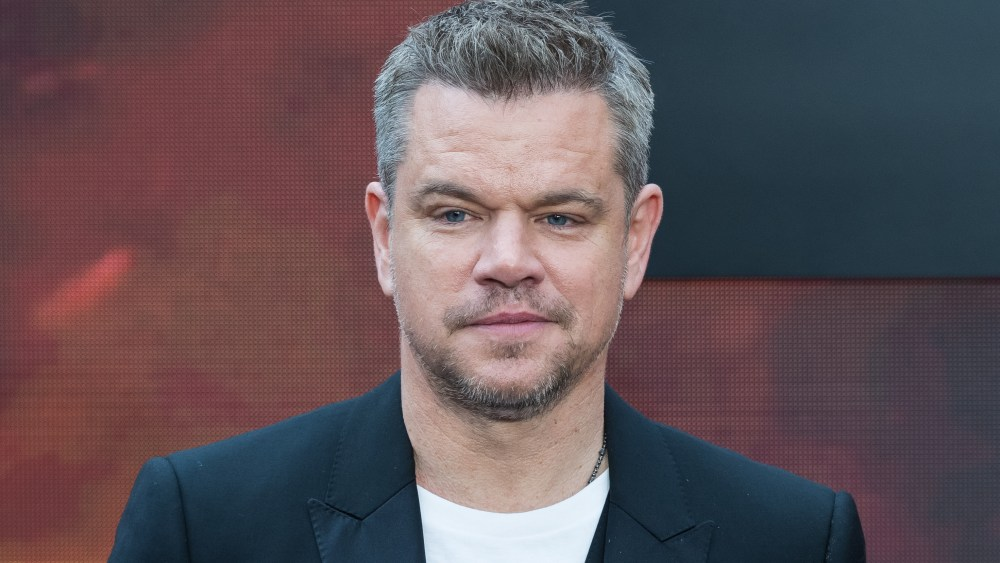
\includegraphics[width=0.9\linewidth]{informatica/ejemploperm_normal}
		\caption{Imagen original}
	\end{subfigure}
	\begin{subfigure}[t]{0.45\textwidth}
		\centering
		
\includegraphics[width=0.9\linewidth]{informatica/ejemploperm_permutada}
		\caption{Imagen original tras aplicar una permutación aleatoria de las posiciones de los \textit{pixels}}
	\end{subfigure}
	\caption{Tenemos que considerar la estructura local de la imagen. La posición de los \textit{pixels} y su vecindario contiene una información fundamental de la que no podemos prescindir. Por tanto, los parches deben contener vecindarios de \textit{pixels}, aunque tengamos distintas estrategias para escoger estos vecindarios.}
	\label{img:desordenar_pixeles_repetida_mates}
\end{figure}

Para decidir la etiqueta de un elemento, consideramos $Y$ \textbf{funciones de puntuación}:

\begin{equation}
	\conjunto{h_y: \mathcal{X} \to \R \dspace / \dspace y \in \mathcal{Y}}.
\end{equation}

\textbf{NOTA PARA JAVIER}: aquí me marcaste debajo de $Y$ y de $\mathcal{Y}$. Escribo $Y$ funciones de puntuación y luego $y \in \mathcal{Y}$ porque he definido $\mathcal{Y} := \deltaset{Y}$. No sé si esta definición aporta poco y lía más que otra cosa, en cuyo caso creo que es mejor quitar la definición de $\mathcal{Y} := \deltaset{Y}$. O si simplemente crees que es mejor que escoja una tipografía o letras que líen menos.
\todo{Borrar esta nota para Javier}

Con esto, dado un elemento $X \in \mathcal{X}$, lo clasificaremos buscando la etiqueta cuya función de puntuación sea máxima, es decir:

$$\hat{y} := \underset{y \in \mathcal{Y}}{argmax} \dspace h_y(X).$$

Por tanto, nuestro \textbf{espacio de hipótesis} es el conjunto de funciones $\Gamma := \conjunto{f: \mathcal{X} \to \R}$. Tanto en la práctica con modelos reales de aprendizaje automático como en nuestras dos modelizaciones, trabajamos en un subconjunto $\tilde{\Gamma} \subseteq \Gamma$ de funciones de puntuación, implementables o bien por el modelo de \textit{machine learning} o bien por nuestra modelización teórica.

\section{Espacio de hipótesis general} \label{sec:espacio_hipotesis_general}
\todo{JMERI: leer de nuevo esta sección completa, porque es muy liosa, repito cosas, introduzco cosas donde no debería. Mirar los contenidos que he borrado}

Nuestro objetivo en esta sección es justificar la elección de las funciones $h_y$ que conformarán el espacio de hipótesis sobre el que trabajaremos. En la \sectionref{sec:repr_funciones_puntuacion} mostramos cuál es la elección final basada en el desarrollo previo. Usaremos ciertos hechos básicos sobre análisis funcional que hemos introducido en la \sectionref{sec:preliminares_funcional}.

\subsection{Planteamiento para construir el espacio de hipótesis} \label{sec:justificacion_func_repr}

Recordemos que los datos de entrada viven en el espacio $\mathcal{X} = (\R^s)^N$ y que, para cada entrada $X \in \mathcal{X}$, tomamos como salida la etiqueta $\hat{y} \in \mathcal{Y}$ que maximice su función de puntuación asociada, que venía dada como:

\begin{equation}
	\hat{y} := \underset{y \in \mathcal{Y}}{argmax} \dspace h_y(X).
\end{equation}

Por lo tanto, buscamos \textbf{construir un espacio de hipótesis} $\mathcal{H} \subseteq L^2((R^s)^N)$ donde elegir nuestras funciones de puntuación. Dicha elección influirá en los modelos de aprendizaje que podamos desarrollar.

Comenzaremos tomando un conjunto de funciones $\conjunto{f_d(\nv{x}): \; d \in \N} \subseteq L^2(\R^S)$ de forma que sea total y linealmente independiente. Llamaremos \textbf{funciones de representación} a las funciones de este conjunto. Gracias a la \propref{prop:conservacion_totalidad_indp_lineal_func_prod} sabemos que la familia de funciones producto inducida $\conjunto{(\nv{x_1}, \ldots, \nv{x_n}) \mapsto \prod_{i = 1}^N f_{d_i}(\nv{x_i}) }_{d_1, \ldots, d_N \in \N} \subseteq L^2((\R^S)^N)$ es también total y linealmente independiente. Por ser total, la \propref{prop:conjuntos_totales_epsilon_aproximacion} nos dice que podemos aproximar funciones de $L^2((\R^S)^N)$ arbitrariamente bien con combinaciones lineales finitas de funciones producto. En la \sectionref{sec:funciones_representacion} hemos visto que podemos escoger funciones de base radial \textit{RBF} o neuronas para tomar un conjunto de funciones de representación que sea total, linealmente independiente y además finito.
\todo{JMeri: hacer la prueba de estos dos resultados que menciono, porque mi desarrollo matemático depende de ellos}

\subsection{Representación tensorial}

Con todo lo anterior tenemos $\epsilon$-aproximación a partir de combinaciones lineales finitas de elementos de un conjunto infinito. Vamos a representar esta aproximación con tensores, lo que nos permitirá más tarde trabajar con modelizaciones basadas en descomposiciones tensoriales. Para ello, consideraremos tensores formales $\mathcal{A}^y \in \espaciotensores{N}{\N}$. Esto es, tensores con $N$ modos, cada modo con una dimensión infinita numerable (podemos considerar que tenemos $N$ sucesiones). El papel de estos tensores formales será el de almacenar los coeficientes de la combinación lineal finita dada por la ecuación \eqref{eq:conjuntos_totales_epsilon_aproximacion} y, por lo tanto, los llamaremos \textbf{tensores de coeficientes}. Como esa combinación lineal es finita, nuestro tensor formal tendrá todas las entradas nulas salvo un conjunto finito. Necesitamos usar tensores formales porque tenemos que elegir qué funciones usamos de un conjunto numerable. Y con esto llegamos a:

\begin{equation} \label{eq:hipotesis_en_general}
	h_y(\nv{x_1}, \ldots, \nv{x_N}) \approx \sum_{d_1, \ldots, d_N \in \N} A^y_{d_1, \ldots, d_N} \prod_{i = 1}^N f_{d_i}(\nv{x_i}).
\end{equation}

Como hemos visto que podemos tomar un conjunto de funciones de representación total, linealmente independiente y además finito, es suficiente considerar $\mathcal{A}^y \in \espaciotensores{N}{M}$ para algún $M \in \N$, con lo que el modelo queda:

\begin{equation}
	h_y(\nv{x_1}, \ldots, \nv{x_N}) \approx \sum_{d_1, \ldots, d_N = 1}^{M} \mathcal{A}^y_{d_1, \ldots, d_N} \prod_{i = 1}^N f_{\theta_{d_i}}(\nv{x_i}).
\end{equation}

De esta forma, este modelo será universal. Podemos aproximar arbitrariamente bien cualquier función de puntuación $h_y \in L^2((\R^S)^N)$ con combinaciones lineales, expresadas a partir de la ecuación anterior. Además, como el conjunto de funciones es linealmente independiente, la expresión anterior es única, y nuestro conjunto de funciones actúa de base del espacio. Es decir, una función de puntuación $h_y$ determina únivocamente el tensor de coeficientes $\mathcal{A}^y$, y podemos escribir:

\begin{equation} \label{eq:puntuacion_general}
	h_y(\nv{x_1}, \ldots, \nv{x_N}) = \sum_{d_1, \ldots, d_N = 1}^{M} \mathcal{A}^y_{d_1, \ldots, d_N} \prod_{i = 1}^N f_{\theta_{d_i}}(\nv{x_i}).
\end{equation}

Así, la tarea de aprendizaje consistirá en aprender a partir de los datos de entrenamiento los coeficientes $\theta_1, \ldots, \theta_M$ de las funciones de representación y los tensores de coeficientes $\mathcal{A}^1, \ldots, \mathcal{A}^Y$.

\begin{observacion}
	Usamos la notación $\sum_{d_1, \ldots, d_N = 1}^{M}$ para denotar $\sum_{d_1 = 1}^{M} \sum_{d_2 = 1}^{M} \ldots \sum_{d_N = 1}^{M}$.
\end{observacion}

\subsection{Capa de representación} \label{subs:capa_de_representacion}

En la ecuación \eqref{eq:puntuacion_general} estamos usando las mismas funciones de representación $f_{\theta_1}, \ldots, f_{\theta_M}: \R^s \to \R$ para todas las funciones de puntuación $h_y$. Lo único que cambia entre las distintas funciones de puntuación es el tensor de coeficientes $\mathcal{A}^y$. Nótese además que en la ecuación \refeq{eq:puntuacion_general}, los vectores de entrada $\nv{x_i}$ solo participan en el producto que involucra computar $f_{\theta_{d_i}}(\nv{x_i})$. Por tanto, podemos considerar un paso inicial, que será compartido en los dos modelos que más adelante introduciremos, consistente en computar los valores:

$$\{f_{\theta_d}(\nv{x_i}): \; d \in \deltaset{M},\ i \in \deltaset{N} \}.$$

Una vez que hayamos computado esos $M \cdot N$ valores, ya no necesitamos los vectores $\nv{x_i}$ para nada más. Con esto, es natural considerar que nuestro modelo tenga una primera capa que compute esos valores, a la que llamaremos \textbf{capa de presentación} y que será una capa convolucional con $M$ canales. Por tanto, cada parche de entrada $\nv{x_i} \in \R^s$ acaba siendo representando por un descriptor de longitud $M$. Con esto, en todas las funciones de puntuación los descriptores resultado de la capa de representación serán los mismos. El siguiente diagrama muestra gráficamente cómo actúa la capa de representación, calculando los $N \cdot M$ coeficientes reales que componen los descriptores de dicha capa:

\begin{figure}[!hbtp]
	\centering
	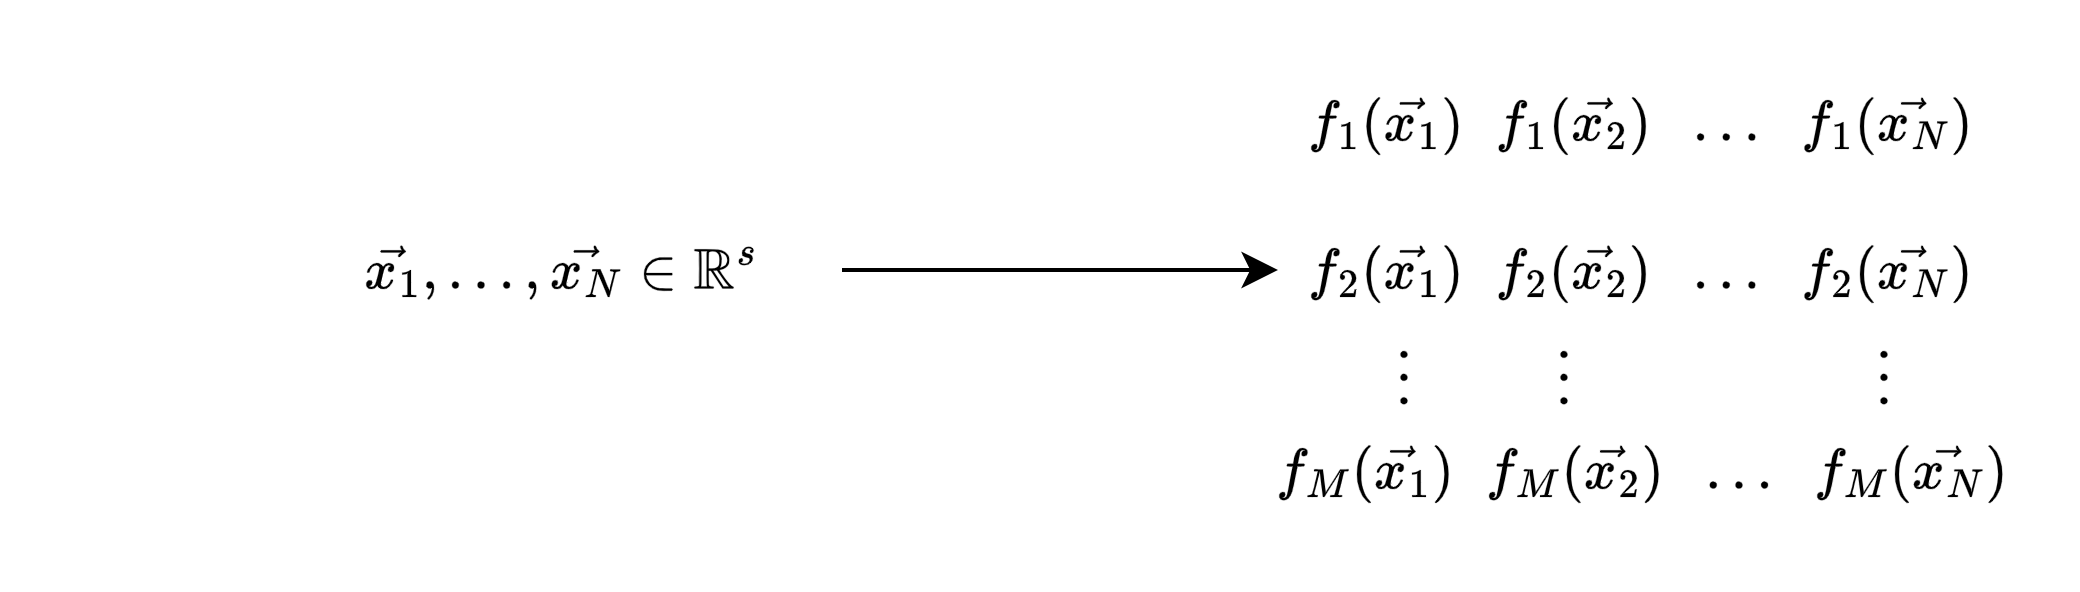
\includegraphics[width=0.8\textwidth]{matematicas/computo_capa_representacion}
	\caption{Ejemplo gráfico sobre cómo actúa la capa de representación. A partir de $N$ parches en $\R^s$, acabamos con $N \cdot M$ coeficientes reales que conformen los descriptores de la capa.}
\end{figure}


\subsection{Ejemplo de cómputo} \label{ejemplo:funcion_puntuacion}

Supongamos que trabajamos con $N = 3, M = 2$. En este caso, una imagen de entrada se compone de los vectores $\nv{x_1}, \nv{x_2}, \nv{x_3} \in \R^s$ (no estamos interesados en el valor de $s \in \N$). Y tenemos dos funciones de representación $f_1, f_2: \R^s \to \R$. El primer paso es computar la capa de representación, que son los $N \cdot M$ coeficientes reales dados por:

\begin{equation}
	\begin{split}
		f_1(\nv{x_1}), f_1(\nv{x_2}), f_1(\nv{x_3}) \\
		f_2(\nv{x_1}), f_2(\nv{x_2}), f_2(\nv{x_3})
	\end{split}
\end{equation}

Y con esto ya podemos expresar nuestra función de puntuación:

\begin{equation}
	\begin{split}
		h_y(\nv{x_1}, \ldots, \nv{x_N}) &= \sum_{d_1, d_2, d_3 = 1}^{2} \mathcal{A}^y_{d_1 d_2 d_3} \prod_{i = 1}^3 f_{d_i}(\nv{x_i}) = A_{111} \; f_1(\nv{x_1}) \; f_1(\nv{x_2}) \; f_1(\nv{x_2}) + A_{112} \; f_1(\nv{x_1}) \; f_1(\nv{x_2}) \; f_2(\nv{x_2}) + \\
		\cdots &+ A_{321} \; f_3(\nv{x_1}) \; f_2(\nv{x_2}) \; f_1(\nv{x_2}) + A_{333} \; f_3(\nv{x_1}) \; f_3(\nv{x_2}) \; f_3(\nv{x_3}).
	\end{split}
\end{equation}

Queda claro que el tensor $\mathcal{A}^y$ contiene los coeficientes que realizan una combinación lineal sobre todos los posibles productos de nuestros $N \cdot M$ valores reales de la capa de representación.

\section{Resumen}

Buscamos resolver una tarea de clasificación de imágenes. Dada una imagen de entrada, debemos asignarle una de las etiquetas $\mathcal{Y} := \{1, \ldots, Y\} = \deltaset{Y}$. Para ello, tomamos la etiqueta cuya función de puntuación asociada $h_y$ sea mayor. Las imágenes de entrada se dividen en parches. Esto es, una imagen viene dada por $N$ vectores $x = (\nv{x_1}, \ldots, \nv{x_N}), \dspace \nv{x_i} \in \R^s \dspace \forall i \in \deltaset{N}$. Elegimos un conjunto finito de funciones de representación que sea total y linealmente independiente. Para ello podemos elegir funciones de base radial \textit{RBF} o neuronas. Aplicando adecuadamente las propiedades del conjunto de funciones, llegamos a la modelización:

\begin{equation}
	h_y(\nv{x_1}, \ldots, \nv{x_N}) = \sum_{d_1, \ldots, d_N = 1}^{M} \mathcal{A}^y_{d_1, \ldots, d_N} \prod_{i = 1}^N f_{\theta_{d_i}}(\nv{x_i}).
\end{equation}

Estudiando esta ecuación nos damos cuenta de que hay un cómputo compartido en todas las funciones de puntuación, que encapsulamos en la capa de representación. Lógicamente, el cómputo de esta capa es compartido para todas las funciones de puntuación.

Las dos arquitecturas que introduciremos más adelante son el resultado de factorizar el tensor de coeficientes $\mathcal{A}^y$ con distintas descomposiciones. Ambas incorporan conceptos claves en la práctica del aprendizaje automático, como la localidad, coeficientes compartidos y \textit{pooling}.

\chapter{Conclusiones} \label{ich:conclusiones}

\todo{Escribir nuestras conclusiones}


% -------------------------------------------------------------------
% BACKMATTER
% -------------------------------------------------------------------

\backmatter % Desactiva la numeración de los capítulos
\pdfbookmark[-1]{Referencias e Índices}{BM-Referencias}

% BIBLIOGRAFÍA
%-------------------------------------------------------------------

\bibliographystyle{alpha}
\begin{small} % Normalmente la bibliografía se imprime en un tamaño de letra más pequeño.
\bibliography{references.bib}
\end{small}

\end{document}
